
%%%%
%%%%  FIGURE 
%%%%
\begin{figure}[h]
\centering
\vbox{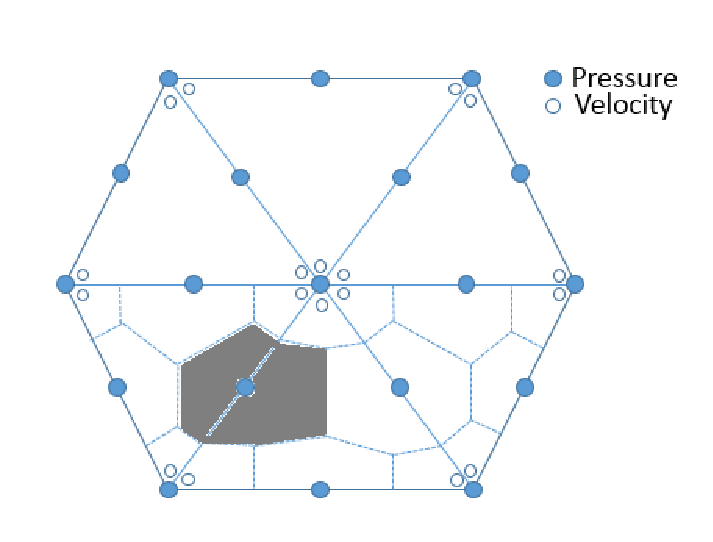
\includegraphics[width=.5\textwidth]{./Pics/P1DGP2.pdf}}
\caption{2D representation of \PN[1]{2} element pairs used in this work. Shaded areas denote control volumes across two contiguous elements. Blue and white circles represent pressure and velocity nodes, respectively.} 
\label{fig:fem_cv}
\end{figure}
\clearpage

%%%%
%%%%  FIGURE
%%%%
\begin{figure}[h]
\centering
\vbox{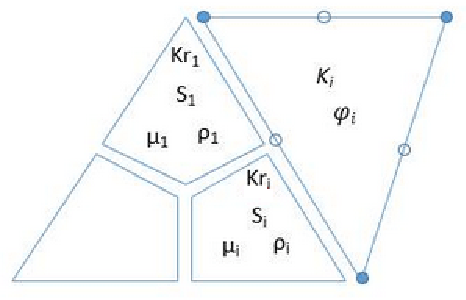
\includegraphics[width=.75\textwidth]{./Pics/element_n.pdf}}
\caption{This is a graphical representation of two different element types. Triangle {\it A} is a representation of the \PN[1]{2} element-pair, whereas triangle {\it B} represents the \PN[1]{1} element-pair. Porosity $\phi_{i}$, permeability {\bf K}$_{i}$, velocity and pressure are primarily represented in FE space whereas scalar fields (such as saturation, density, viscosity etc) are represented in CV space.}
\label{fig:fem_elem}
\end{figure}
\clearpage

%%%%
%%%%  FIGURE 
%%%%
\begin{figure}[h]
\centering
\vbox{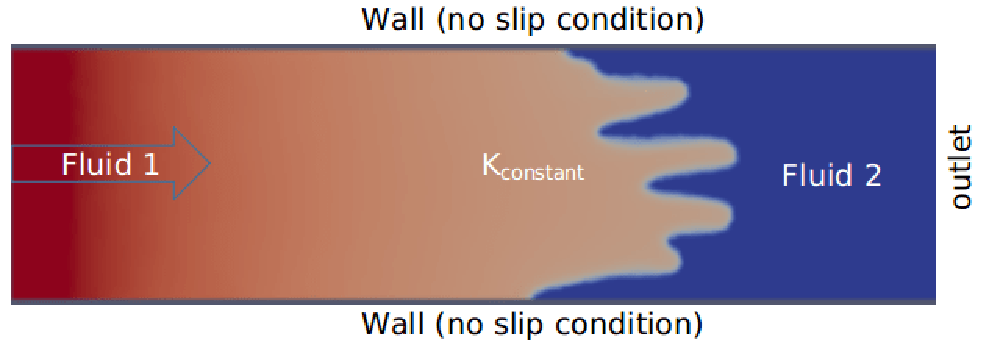
\includegraphics[width=0.75\textwidth]{./Pics/phase_vol_frac_uni_perm_1.pdf}}
\caption{Schematics of formation of flow instabilities during injection of a pure low viscosity fluid (red) into a domain saturated with a second fluid (dark blue). The viscocity ratio of the two fluids is VR=$5$. In this case, the initially piston shape front collapses leading to the formation of several fingers.}
\label{fig:simple_case}
\end{figure}
\clearpage


%%%%
%%%%  FIGURE 
%%%%
\begin{figure}[ht] 
\vbox{
\hbox{\hspace{-0.3cm}
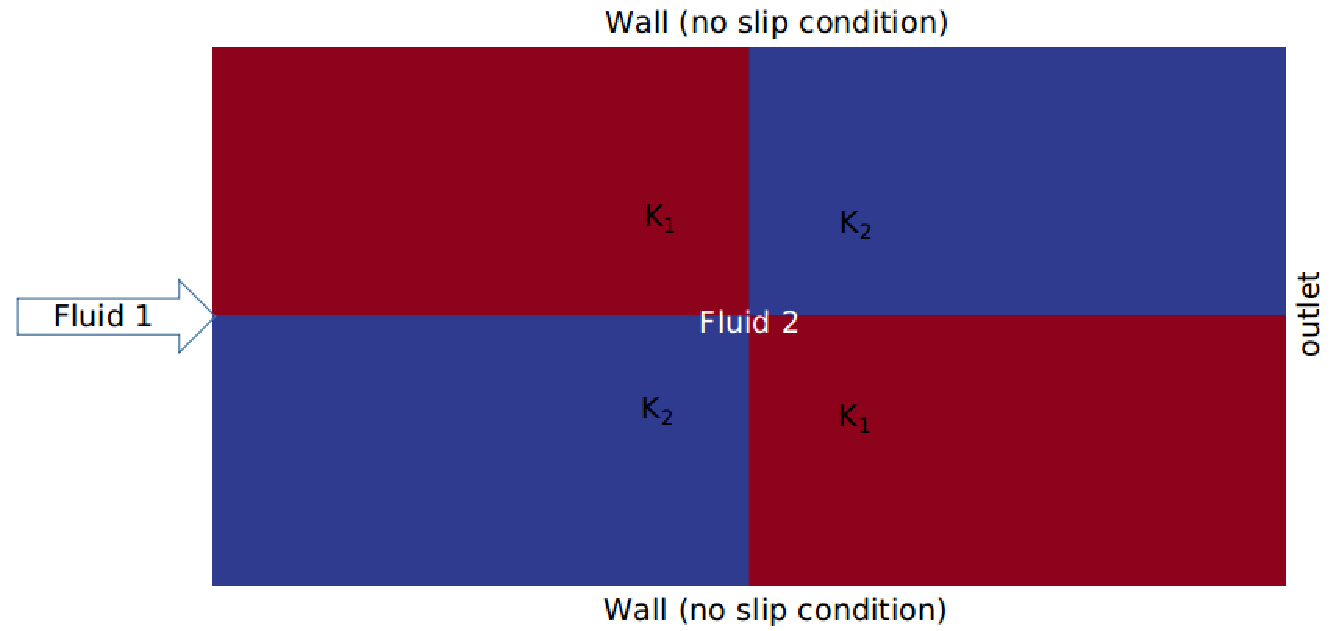
\includegraphics[width=.8\textwidth]{./Pics1/2b2_wi_fine/2b2_whole_in_fine_perm_1.pdf} 
}
\vspace{0.0cm}
\hbox{\hspace{3.5cm} (a) map of permeabilities ($\mathbf{K}$)
}
\vspace{0.25cm}
\hbox{\hspace{1.5cm}
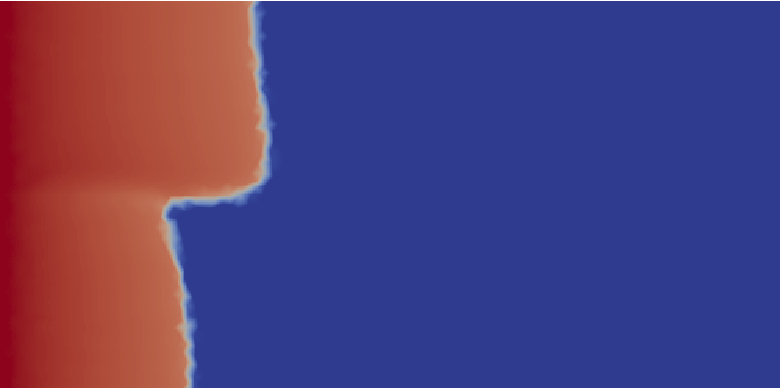
\includegraphics[width=.85\textwidth]{./Pics1/2b2_wi_fine/2b2_whole_in_fine_250_2.pdf}
}
\vspace{0.0cm}
\hbox{\hspace{4.5cm} (b) flow at t=250 
}
\vspace{0.25cm}
\hbox{\hspace{1.5cm}
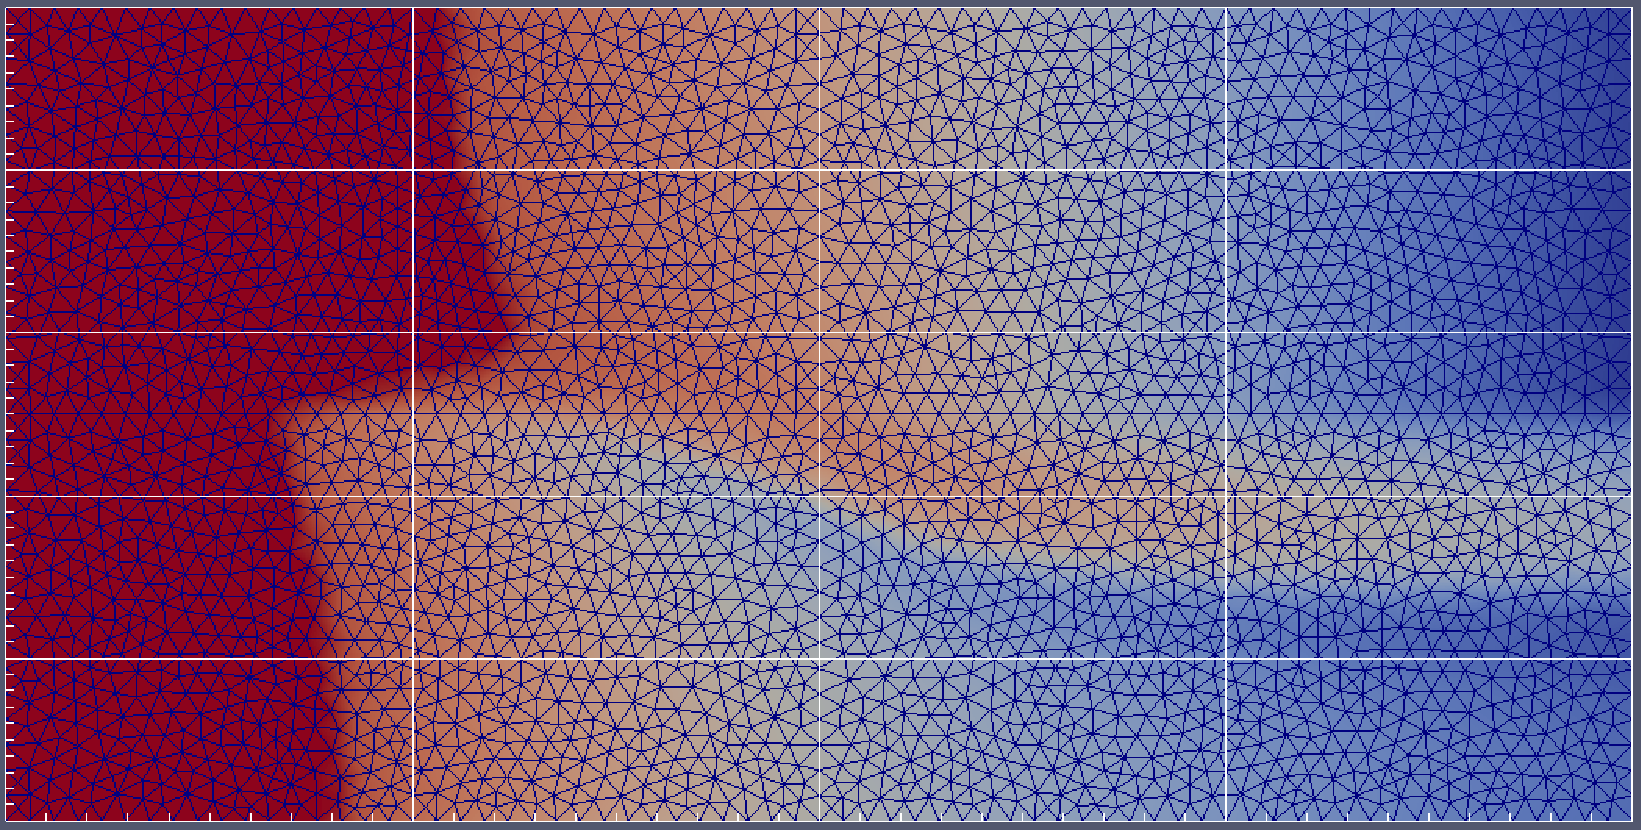
\includegraphics[width=.65\textwidth]{./Pics1/2b2_wi_fine/2b2_whole_in_fine_3000_2.pdf}
}
\vspace{0.0cm}
\hbox{\hspace{4.0cm} (c) flow at t=3000   
}}     
\caption{Model validation of fluid displacement in heterogeneous porous media ({\it VR}=1): (a) the domain is divided into four subdomains with prescribed synthetic permeability, $\mathbf{K}_{1}=1$ and $\mathbf{K}_{2}=2.5$; (b-c) snapshots of saturation (displacing fluid) field at t=$25$s and t=$300$ sec. The domain is discretised with $5960$ \PN[1]{2} elements. }
\label{fem_cv_represent_a}
\end{figure}
\clearpage



%%%%
%%%%  FIGURE
%%%%
\begin{landscape}
\begin{figure}[ht] 
\vbox{\vspace{-1cm}
\hbox{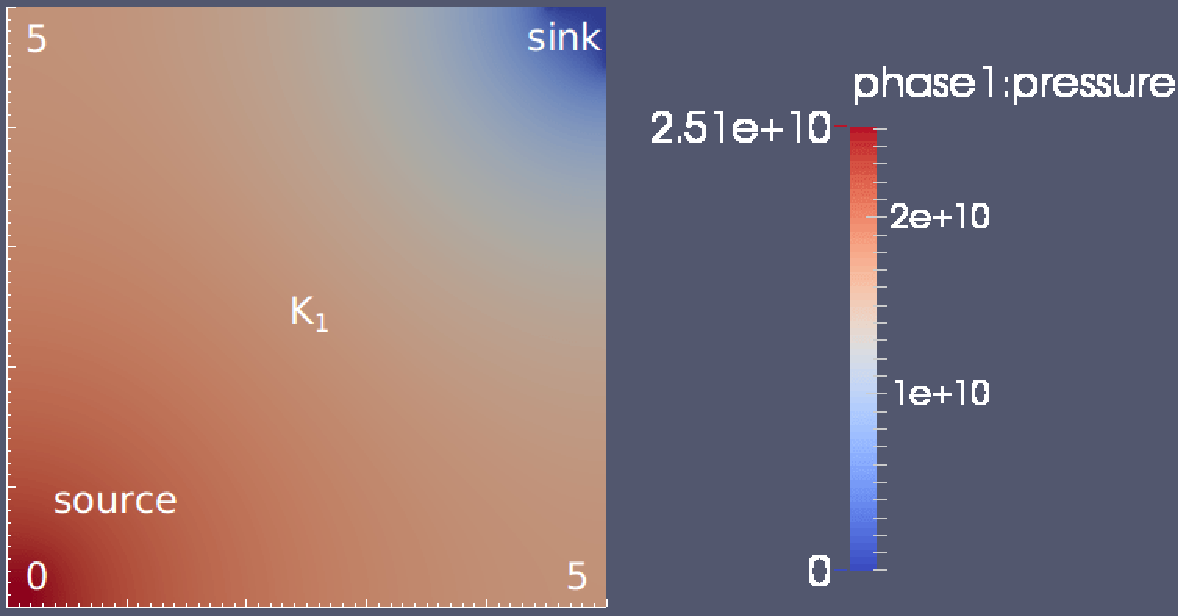
\includegraphics[width=.71\textwidth]{./Pics1/Saffman_homogeneous_MR3/saffman_homo_fixed_2.pdf}
      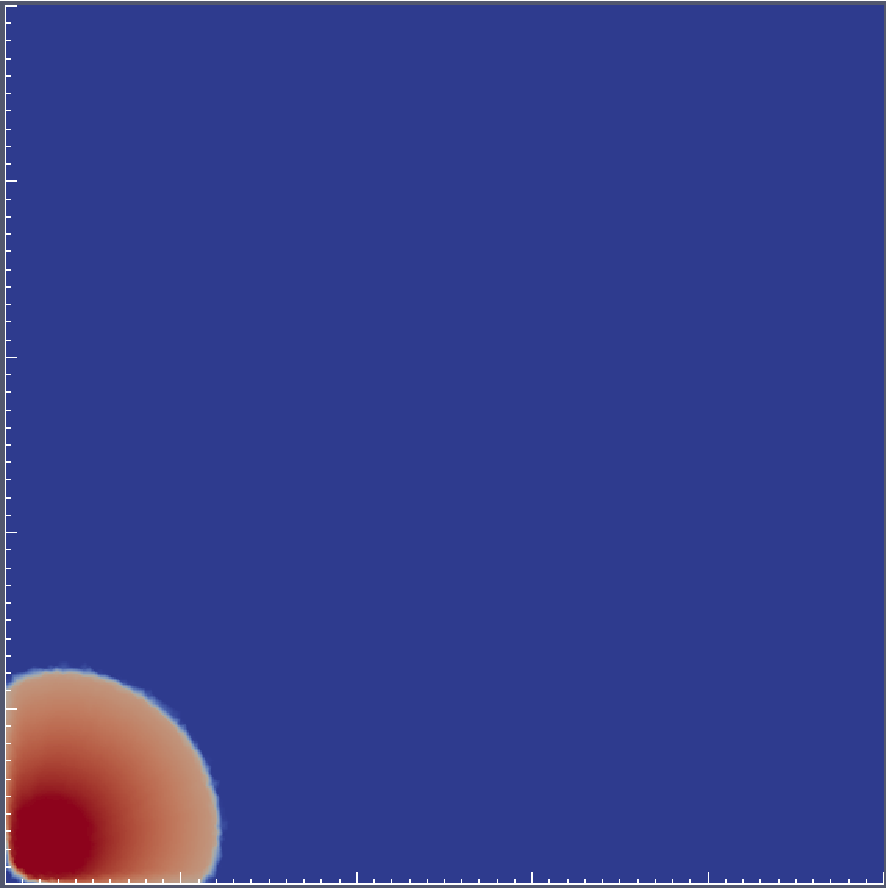
\includegraphics[width=.37\textwidth]{./Pics1/Saffman_homogeneous_MR3/saffman_homo_fixed_250.pdf}
      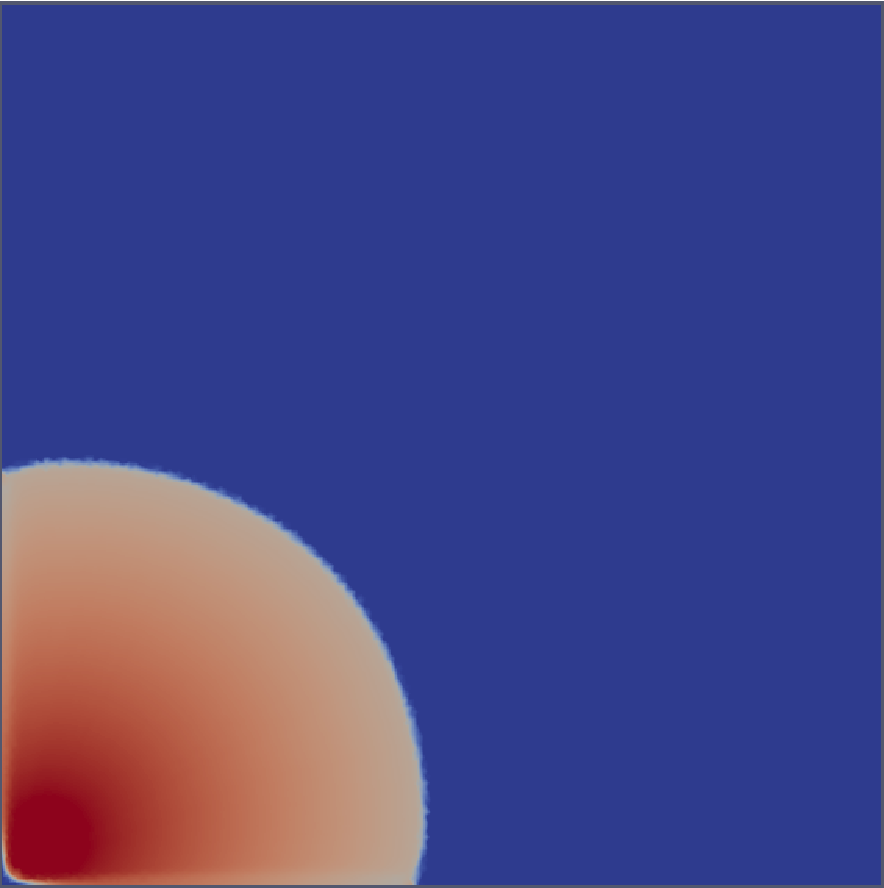
\includegraphics[width=.37\textwidth]{./Pics1/Saffman_homogeneous_MR3/saffman_homo_fixed_1000.pdf}}
\vspace{0.cm}
\hbox{\hspace{2.5cm} (a) pressure at t=0s \hspace{5.cm} (b) t=0.87s \hspace{2.75cm} (c) t=3.54s}
\vspace{0.5cm}
\hbox{
      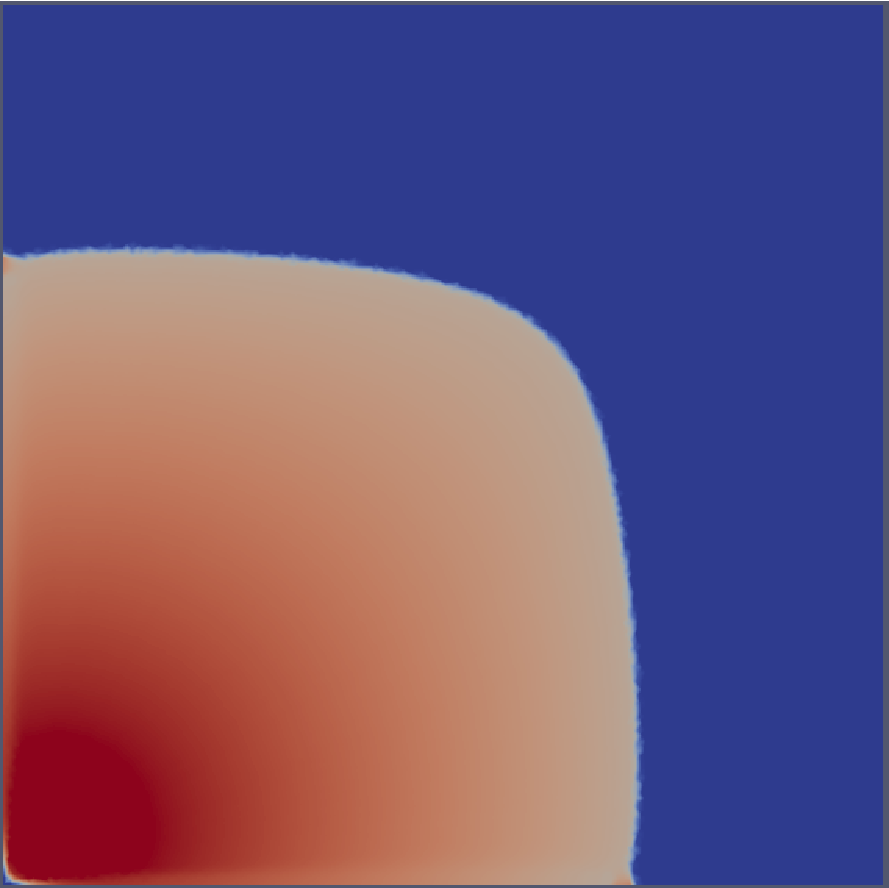
\includegraphics[width=.38\textwidth]{./Pics1/Saffman_homogeneous_MR3/saffman_homo_fixed_2500.pdf}
      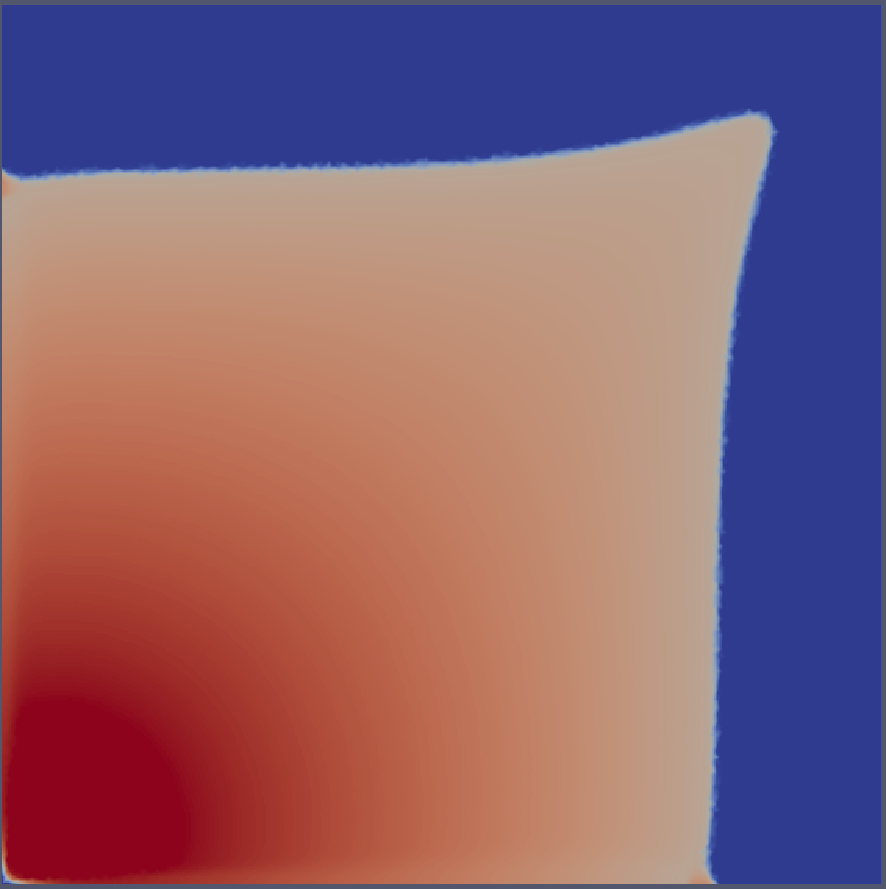
\includegraphics[width=.38\textwidth]{./Pics1/Saffman_homogeneous_MR3/saffman_homo_fixed_3500.pdf} 
      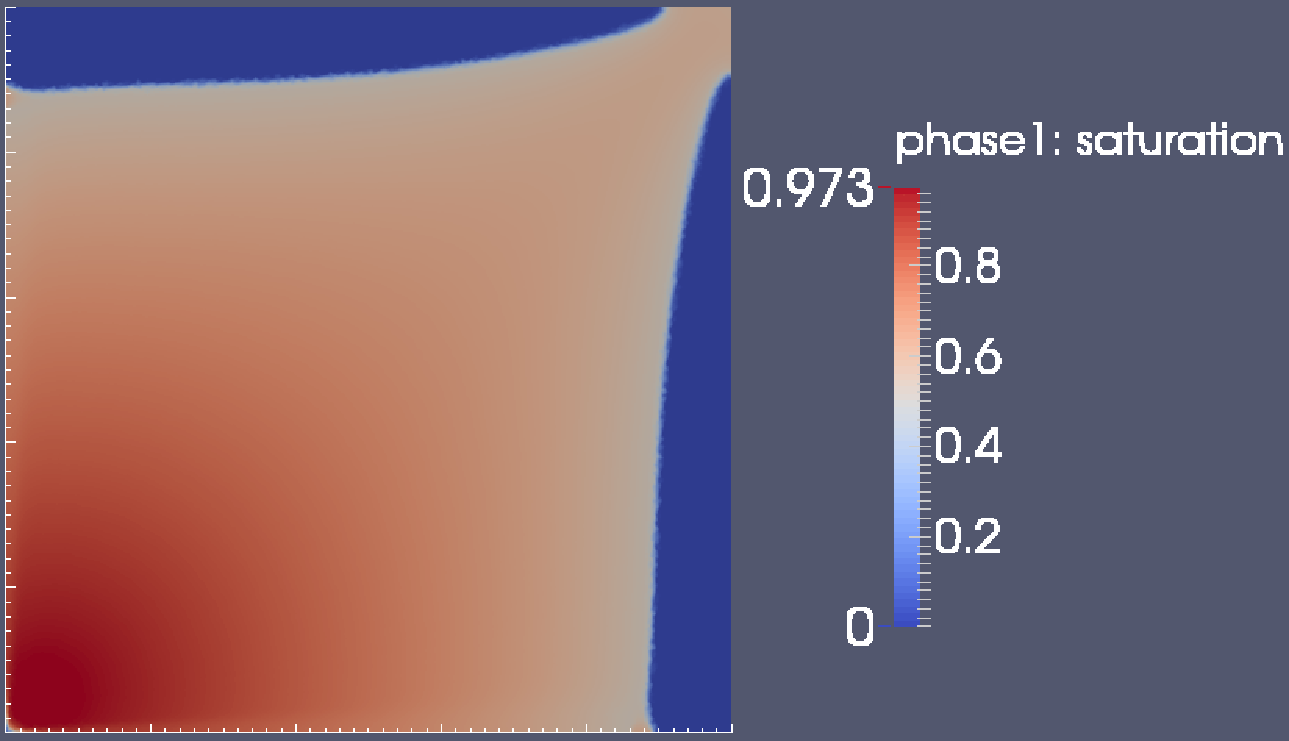
\includegraphics[width=.66\textwidth]{./Pics1/Saffman_homogeneous_MR3/saffman_homo_fixed_end.pdf}}
\vspace{0.cm}
\hbox{ \hspace{1.cm} (d) t=8.86s \hspace{3.0cm} (e) t=12.41s   \hspace{4.0cm} (f) t=17.95s}
\vspace{0.cm}
}   
\caption{Simulated flow in a Hele-Shaw cell $\left(\text{{\it VR}=3, {\bf K}=10}^{-10}\text{cm}^{2}\right)$: (a) initial pressure profile $\left(\text{in g.cm}^{-1}\text{.s}^{-2}\right)$ with source and sink regions are explicitly shown along with dimensions (in cm); (b-f) snapshots of wetting phase saturation showing flow profile as the simulation evolves. The domain contains $26313$ \PN[1]{2} triangular elements.}
\label{fig:homoheleshaw_VN3}
\end{figure}
\end{landscape}
\clearpage



%%%%
%%%%  FIGURE
%%%%
\begin{landscape}
\begin{figure}[ht] 
\vbox{\vspace{-1cm}
\hbox{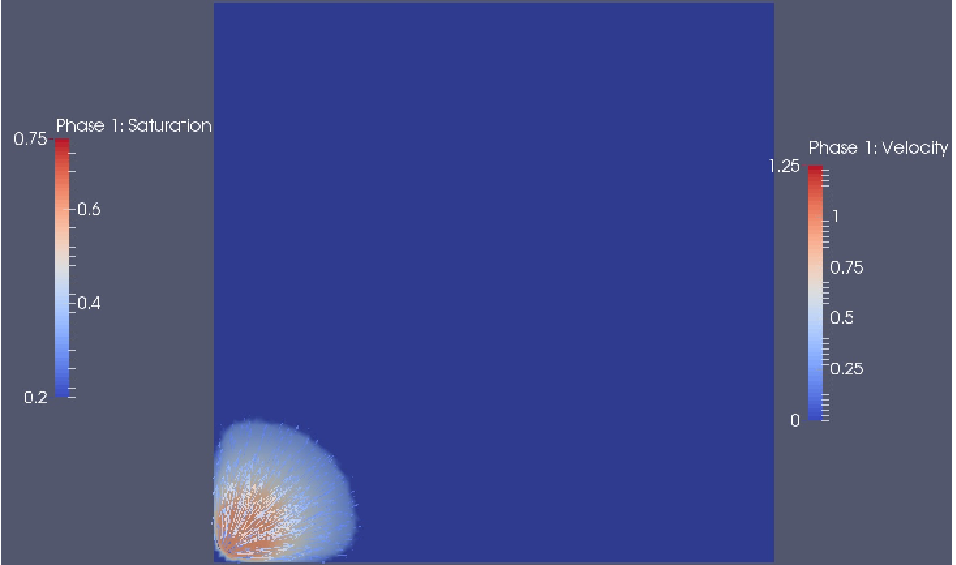
\includegraphics[width=.9\textwidth, height=0.5\textwidth]{./Pics1/Saffman_homogeneous_VR10/ST_Homog_VR10_D201c.pdf}
\hspace{0.5cm}      
      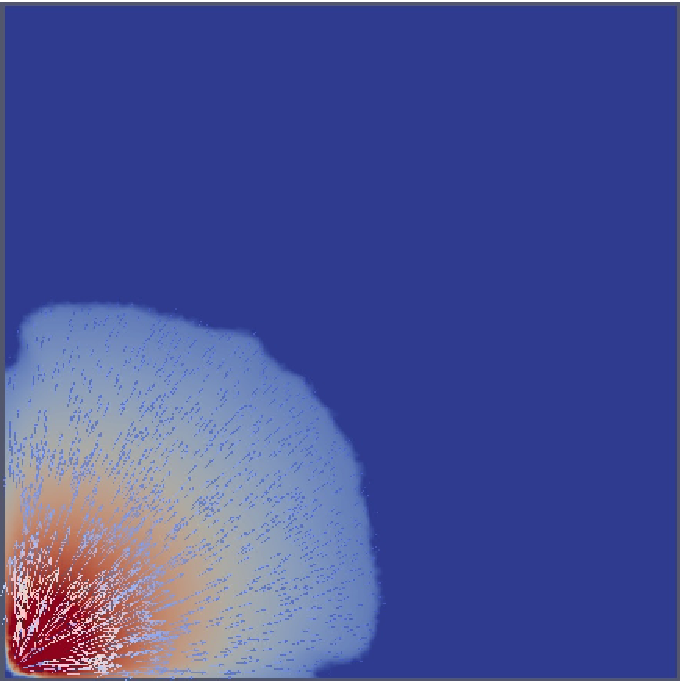
\includegraphics[width=.5\textwidth]{./Pics1/Saffman_homogeneous_VR10/ST_Homog_VR10_D1001c.pdf}}
\vspace{0.cm}
\hbox{\hspace{5.cm} (a) t=0.66s \hspace{8.cm} (b) t=3.43s }
\vspace{0.5cm}
\hbox{
      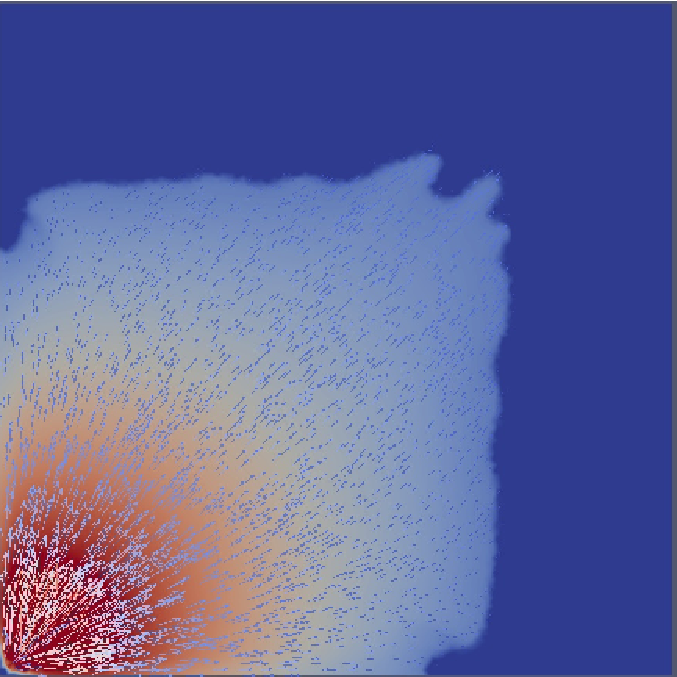
\includegraphics[width=.51\textwidth]{./Pics1/Saffman_homogeneous_VR10/ST_Homog_VR10_D2001c}
      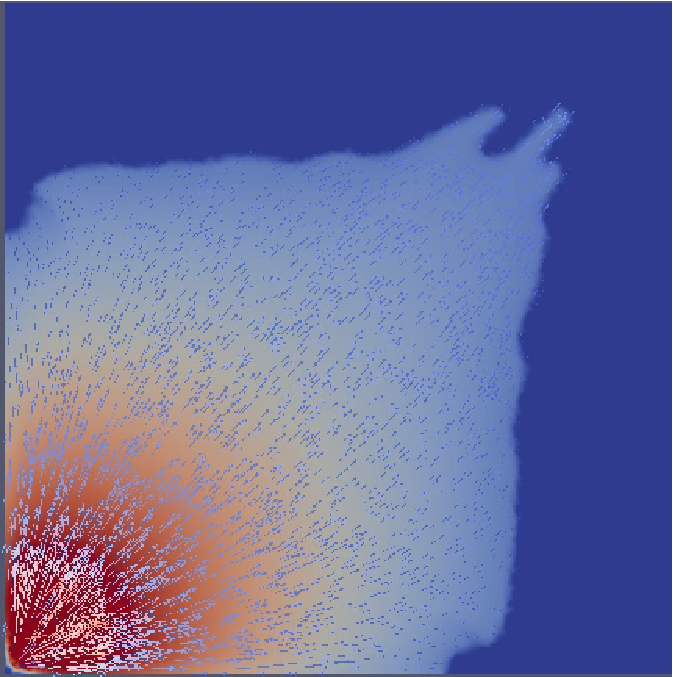
\includegraphics[width=.5\textwidth]{./Pics1/Saffman_homogeneous_VR10/ST_Homog_VR10_D2201c}
      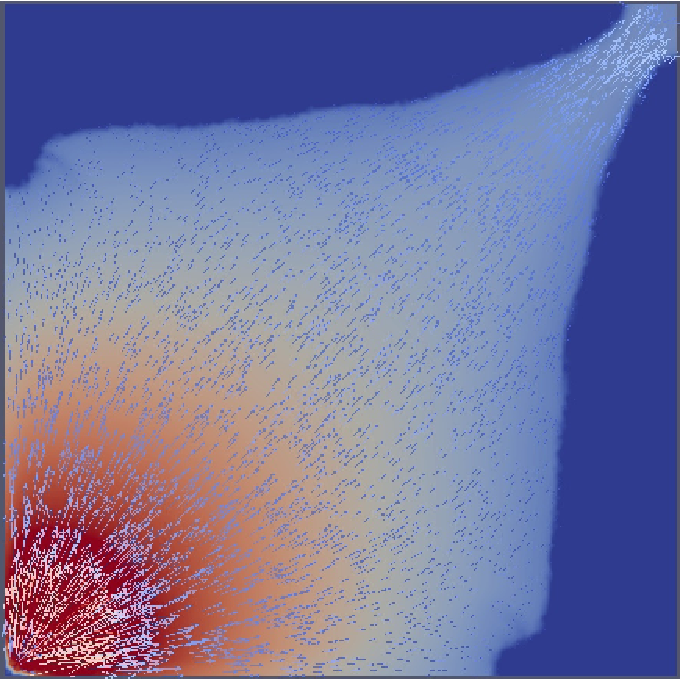
\includegraphics[width=.51\textwidth]{./Pics1/Saffman_homogeneous_VR10/ST_Homog_VR10_D3001c}}
\vspace{0.cm}
\hbox{ \hspace{2.cm} (c) t=6.92s \hspace{4.5cm} (d) t=7.61s \hspace{5.cm} (e)t=10.00s}
\vspace{0.cm}
}   
\caption{Simulated flow in a Hele-Shaw cell $\left(\text{{\it VR}=10, {\bf K}=10}^{-10}\text{cm}^{2}\right)$: snapshots of overlapped wetting phase saturation and velocity vectors showing flow profile as the simulation evolves. The domain contains $26313$ \PN[1]{2} triangular elements.}
\label{fig:homoheleshaw_VN10}
\end{figure}
\end{landscape}
\clearpage

%%%%
%%%%  FIGURE
%%%%
\begin{landscape}
\begin{figure}[ht] 
\vbox{\vspace{-1cm}
\hbox{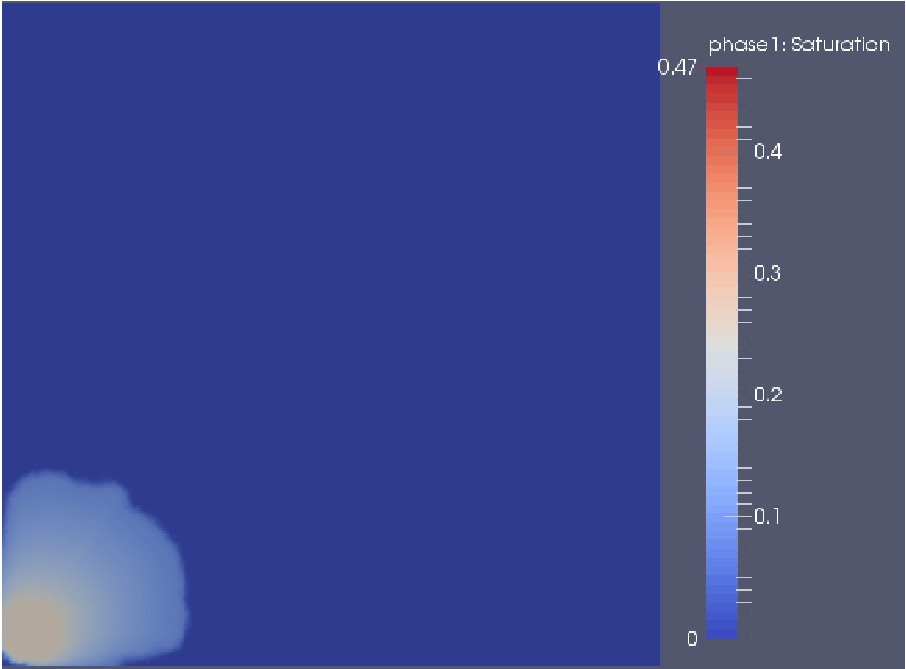
\includegraphics[width=.9\textwidth, height=0.5\textwidth]{./Pics1/Saffman_homogeneous_VR150/ST_Homog_VR150_D300b}
\hspace{0.5cm}      
      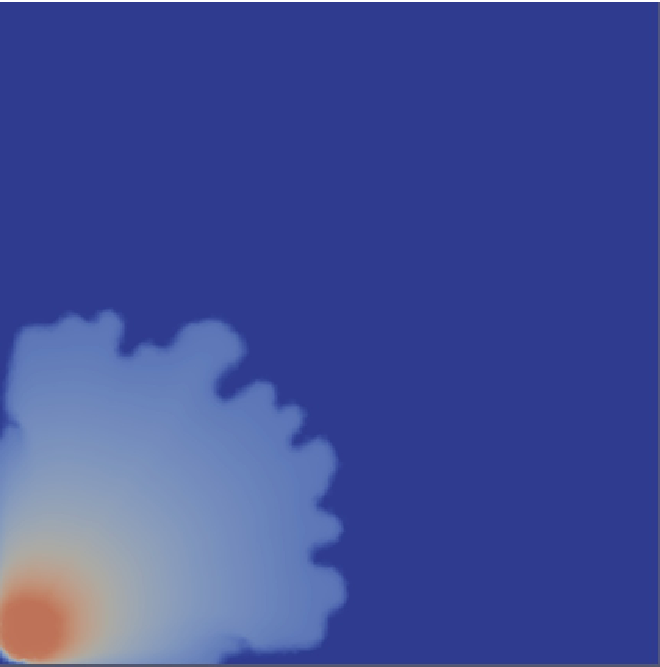
\includegraphics[width=.5\textwidth]{./Pics1/Saffman_homogeneous_VR150/ST_Homog_VR150_D1600b}}
\vspace{0.cm}
\hbox{\hspace{5.cm} (a) t=0.27s \hspace{8.cm} (b) t=0.94s }
\vspace{0.5cm}
\hbox{
      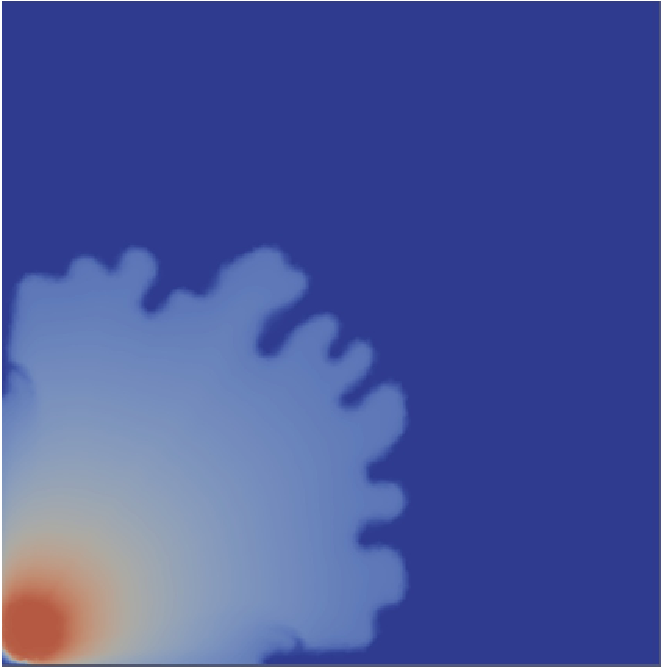
\includegraphics[width=.5\textwidth]{./Pics1/Saffman_homogeneous_VR150/ST_Homog_VR150_D2700b}
      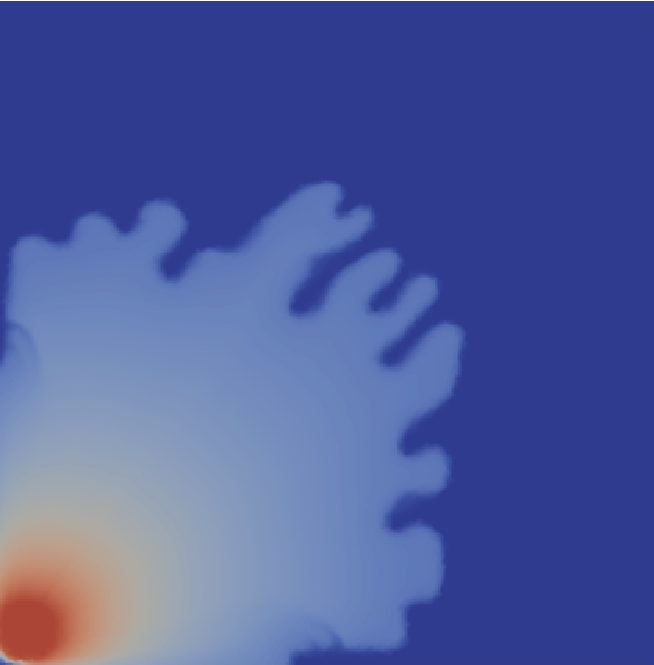
\includegraphics[width=.5\textwidth]{./Pics1/Saffman_homogeneous_VR150/ST_Homog_VR150_D4000b}
      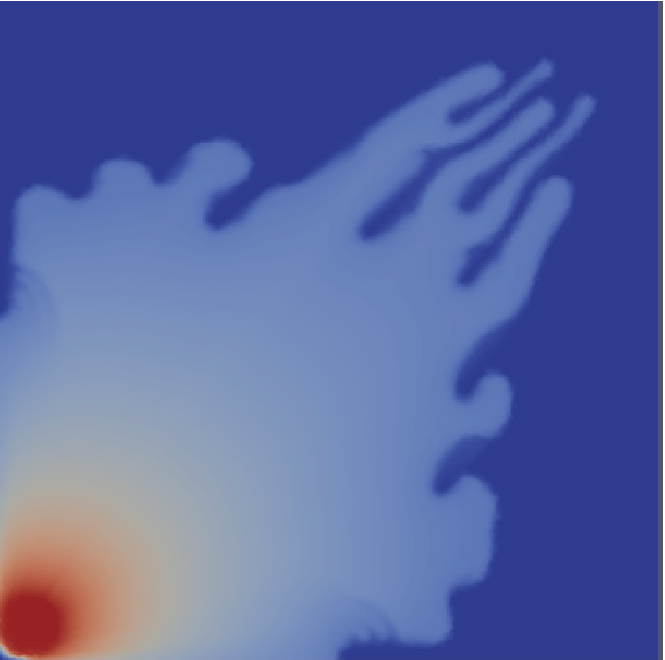
\includegraphics[width=.51\textwidth]{./Pics1/Saffman_homogeneous_VR150/ST_Homog_VR150_D7000b}}
\vspace{0.cm}
\hbox{ \hspace{2.cm} (c) t=1.32s \hspace{4.5cm} (d) t=1.70s \hspace{5.cm} (e)t=2.31s}
\vspace{0.cm}
}   
\caption{Simulated flow in a Hele-Shaw cell $\left(\text{{\it VR}=150, {\bf K}=10}^{-10}\text{cm}^{2}\right)$: snapshots of wetting phase saturation showing flow profile as the simulation evolves. The domain contains $26313$ \PN[1]{2} triangular elements.}
\label{fig:homoheleshaw_VN150}
\end{figure}
\end{landscape}
\clearpage


%%%
%%% FIGURE XXXXXX
%%%
\begin{landscape}
  \begin{figure}[ht]
  \vbox{\vspace{-.5cm}
      \hbox{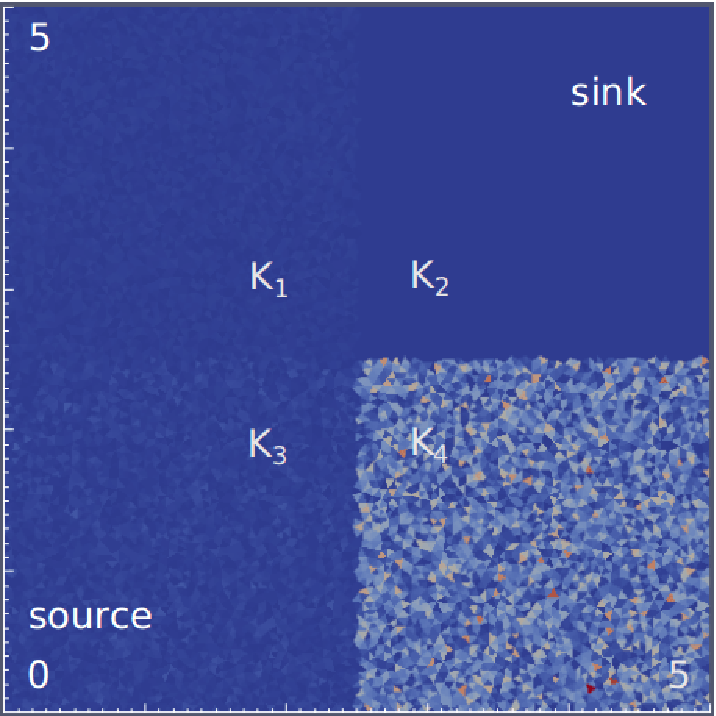
\includegraphics[width=.4\textwidth]{./Pics1/Saffman_heterogeneous/saffman_heter_fixed_1.pdf}
            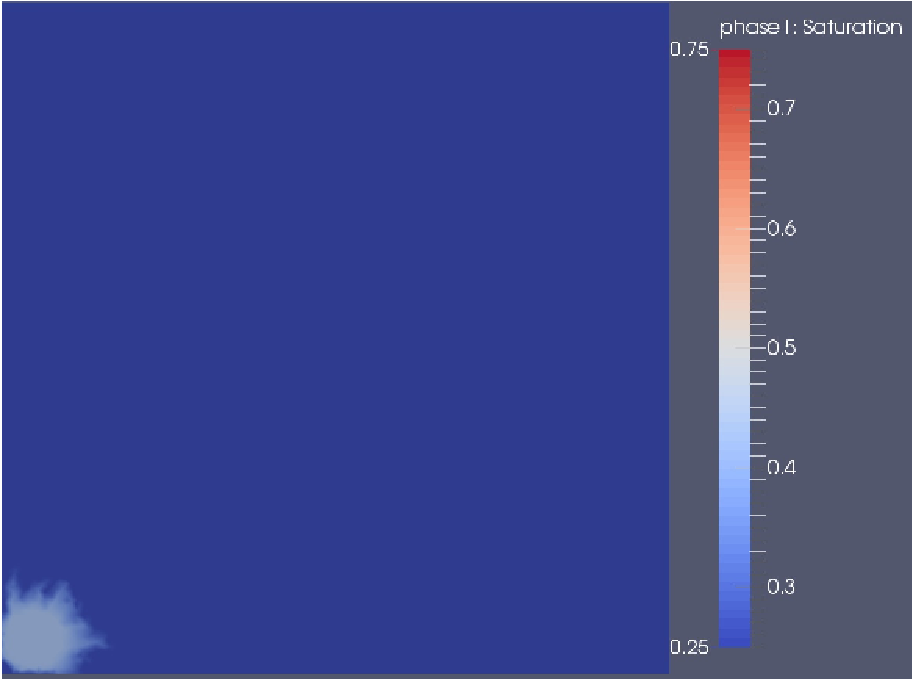
\includegraphics[width=.55\textwidth, height=.4\textwidth]{./Pics1/Saffman_heterogeneous_VR10/ST_Heterog_VR10_D200Hb.pdf} 
            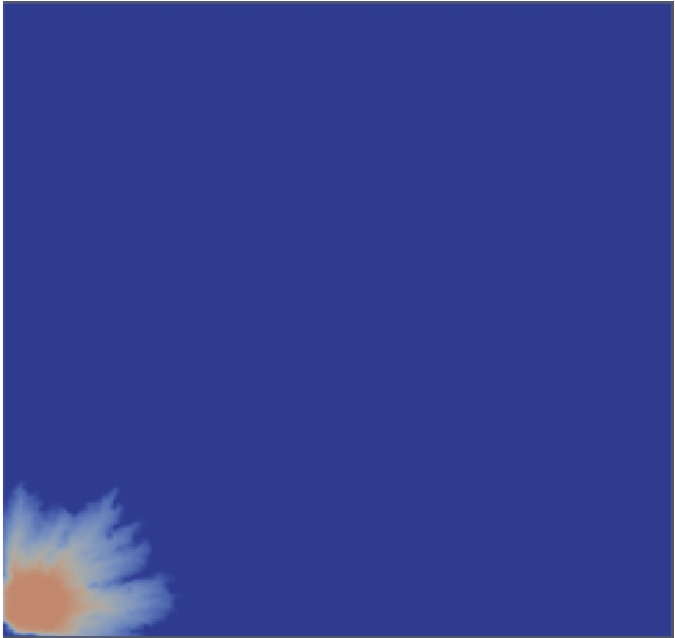
\includegraphics[width=.42\textwidth]{./Pics1/Saffman_heterogeneous_VR10/ST_Heterog_VR10_D900Hb.pdf} }
      \hbox{\hspace{1.0cm} (a) permeability map \hspace{3.cm} (b) t=0.19s \hspace{4.0cm} (c) t=0.63s}
      \vspace{0.5cm}
      \hbox{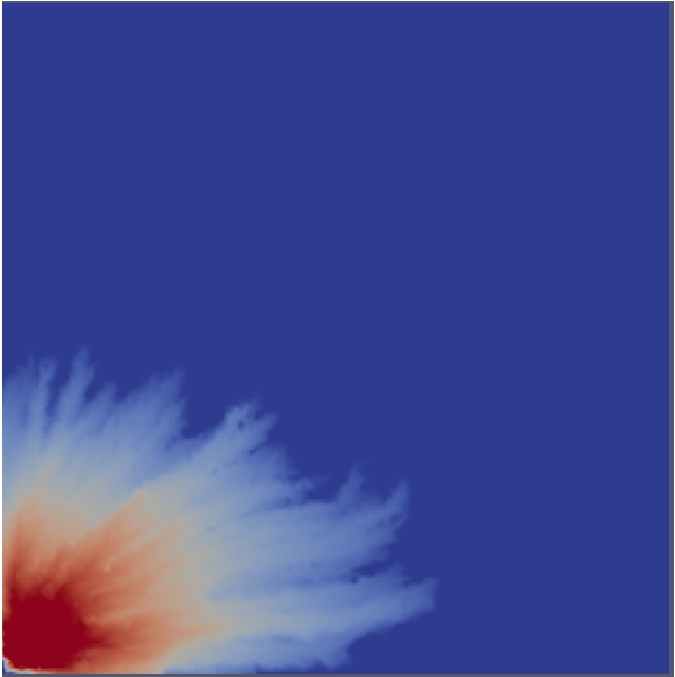
\includegraphics[width=.45\textwidth]{./Pics1/Saffman_heterogeneous_VR10/ST_Heterog_VR10_D5000Hb.pdf}
            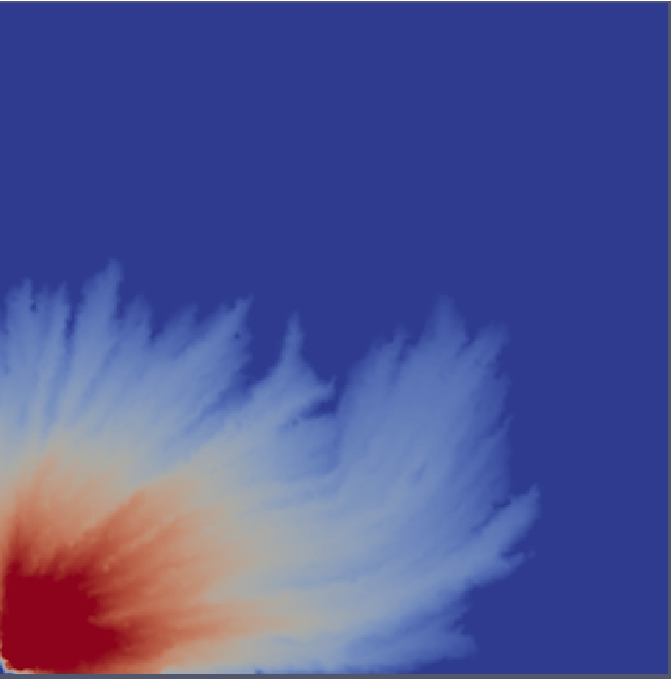
\includegraphics[width=.45\textwidth]{./Pics1/Saffman_heterogeneous_VR10/ST_Heterog_VR10_D8000Hb.pdf}
            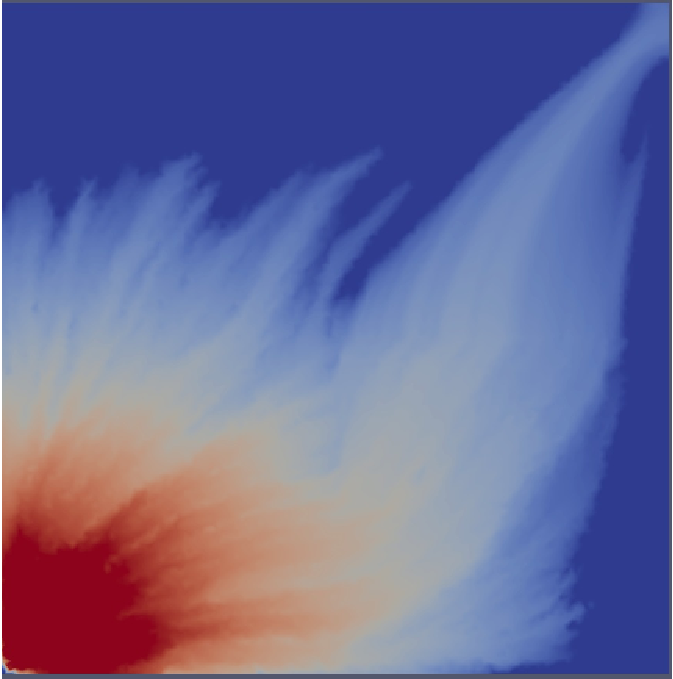
\includegraphics[width=.45\textwidth]{./Pics1/Saffman_heterogeneous_VR10/ST_Heterog_VR10_D13800Hb.pdf} }
      \hbox{\hspace{2.cm} (d) t=3.41s \hspace{3.5cm} (e) t= 5.54s\hspace{4.5cm} (f) t=9.77s }}
\caption{Simulated flow in a modified Hele-Shaw cell with {\it VR}=10: (a) permeability distribution $\left(\text{10}^{-10}\le\mathbf{K}_{1}\le\text{5}\times\text{10}^{-10}\right.$, {\bf K}$_{2}$=10$^{-10}$, 10$^{-11}\le\mathbf{K}_{3}\le$ 5$\times$10$^{-10}$ and 10$^{-12}\le\mathbf{K}_{4}\le$ 5$\times$10$\left.^{-10}\text{ cm}^{2}\right)$; (b-f) snapshots of saturation profile during 9.77 seconds of simulation. The domain contains 26313 \PN[1]{2} element-pairs.}
\label{fig:HeleShawHeter_VR10}
\end{figure}
\end{landscape}
\clearpage

%%%
%%% FIGURE XXXXXX
%%%
\begin{landscape}
  \begin{figure}[ht]
  \vbox{\vspace{-.5cm}
      \hbox{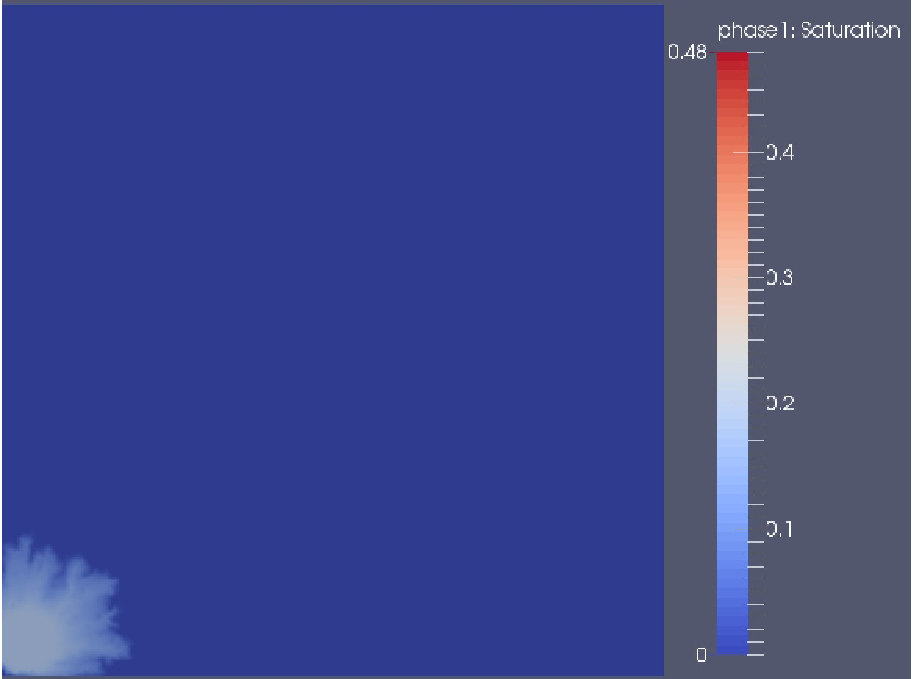
\includegraphics[width=.65\textwidth, height=.46\textwidth]{./Pics1/Saffman_heterogeneous_VR150/ST_Heterog_VR150_D200Hb.pdf} 
            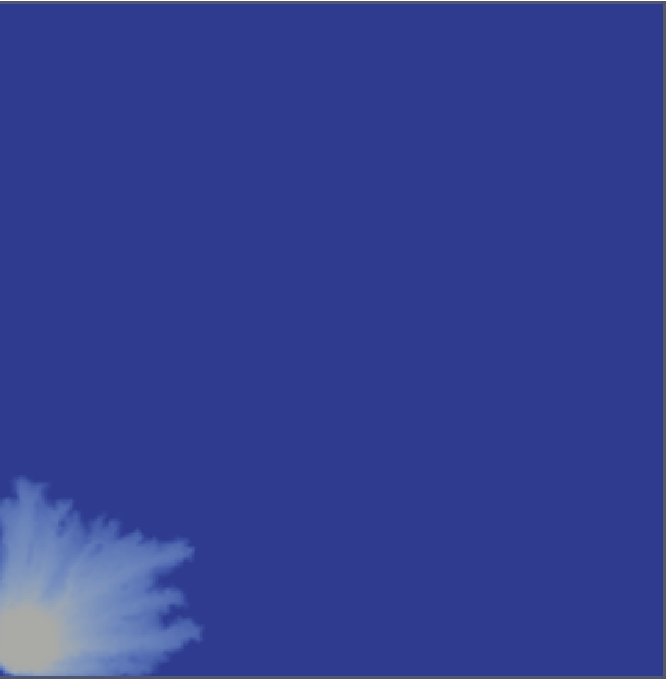
\includegraphics[width=.45\textwidth]{./Pics1/Saffman_heterogeneous_VR150/ST_Heterog_VR150_D500Hb.pdf}
            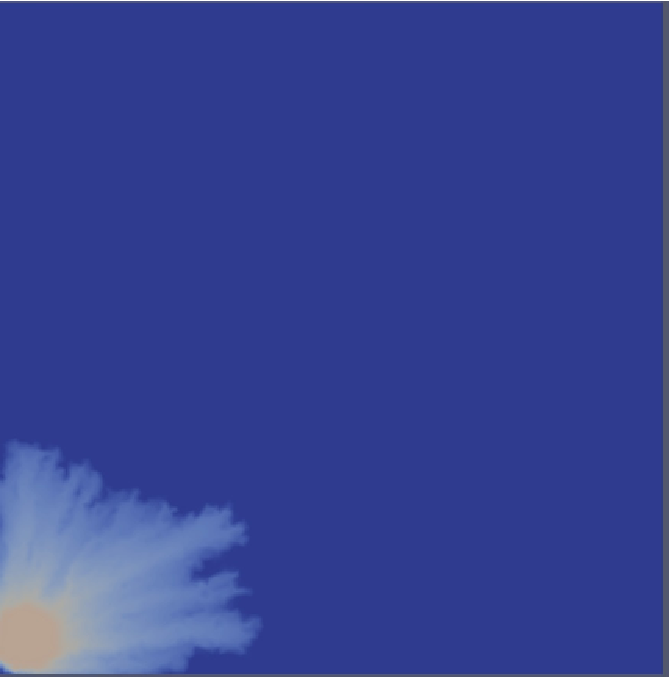
\includegraphics[width=.45\textwidth]{./Pics1/Saffman_heterogeneous_VR150/ST_Heterog_VR150_D800Hb.pdf} }
      \hbox{\hspace{2.0cm} (a) t=0.10s \hspace{6.cm} (b) t=0.24ss \hspace{4.cm} (c) t=0.37s}
      \vspace{0.5cm}
      \hbox{\hspace{.5cm} 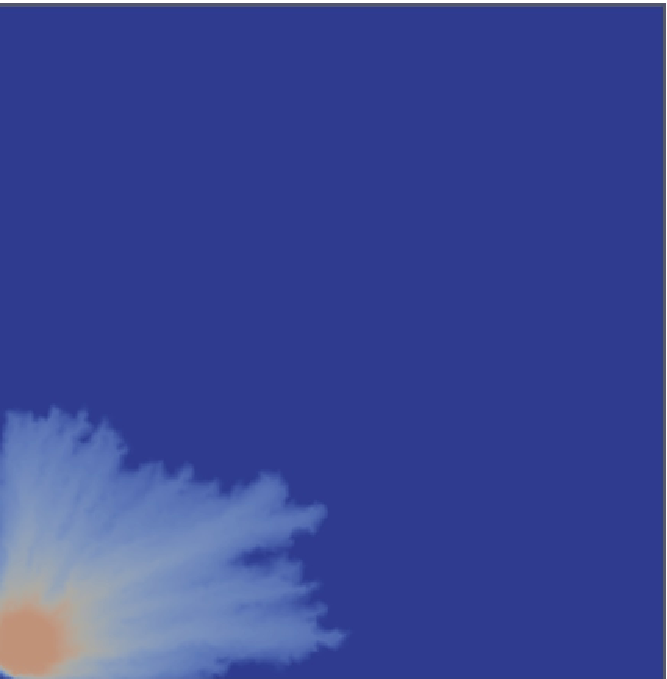
\includegraphics[width=.45\textwidth]{./Pics1/Saffman_heterogeneous_VR150/ST_Heterog_VR150_D1500Hb.pdf}
            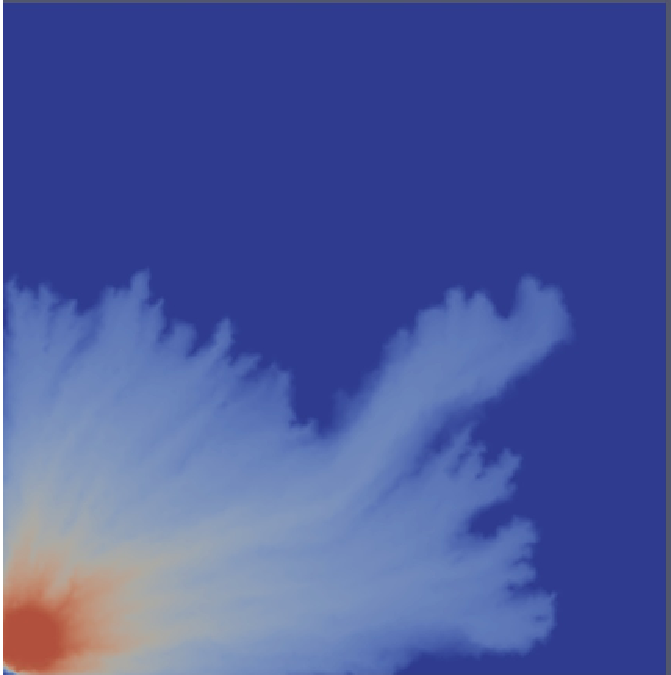
\includegraphics[width=.45\textwidth]{./Pics1/Saffman_heterogeneous_VR150/ST_Heterog_VR150_D5000Hb.pdf}
            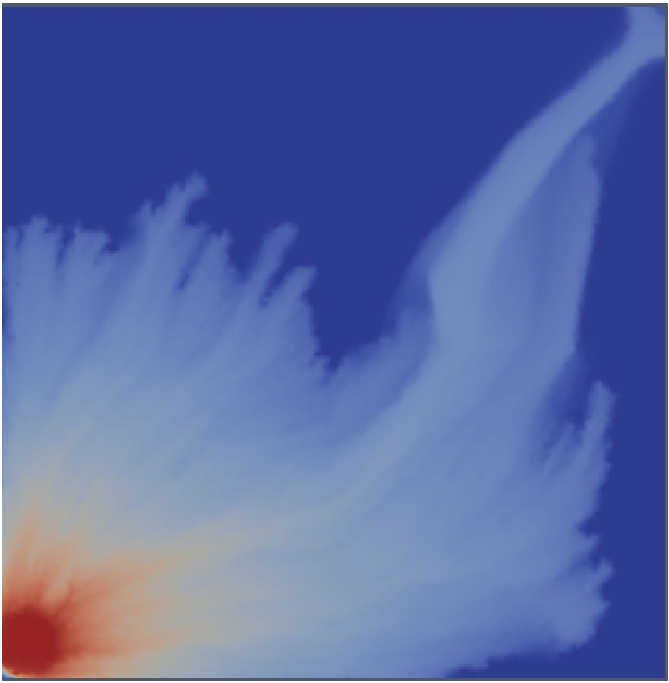
\includegraphics[width=.45\textwidth]{./Pics1/Saffman_heterogeneous_VR150/ST_Heterog_VR150_D8000Hb.pdf} }
      \hbox{\hspace{3.cm} (d) t=0.59s \hspace{3.cm} (e) t= 1.61s\hspace{4.cm} (f) t=2.50s }}
\caption{Simulated flow in a modified Hele-Shaw cell with {\it VR}=150: snapshots of saturation profile during 2.50 seconds of simulation. Permeability distribution used in this simulation was the same as shown in Fig.~\ref{fig:HeleShawHeter_VR10}a. The domain contains 26313 \PN[1]{2} element-pairs.}
\label{fig:HeleShawHeter_VR150}
\end{figure}
\end{landscape}
\clearpage


%%%%
%%%%  FIGURE
%%%%
\begin{figure}[ht]
\vbox{
\hbox{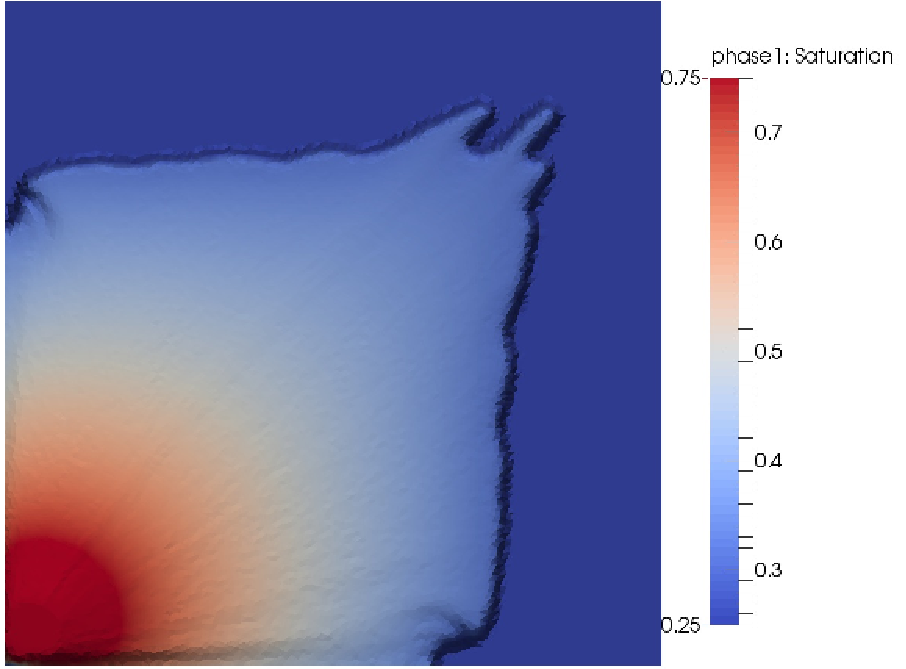
\includegraphics[width=.5\textwidth]{./Pics1/Saffman_homogeneous_VR10/ST_Homog_VR10_D2201_W2b.pdf}
       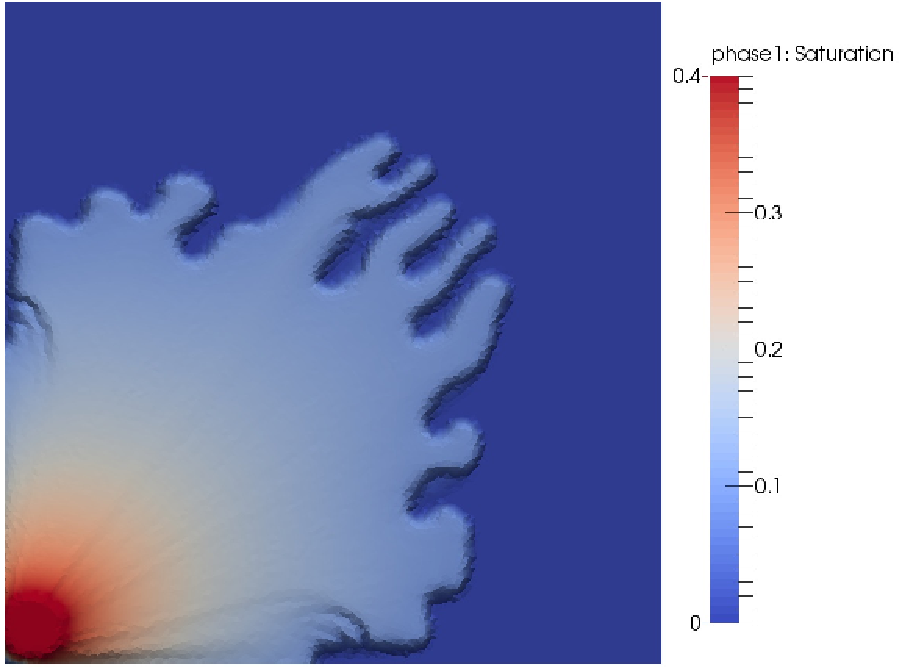
\includegraphics[width=.5\textwidth]{./Pics1/Saffman_homogeneous_VR150/ST_Homog_VR150_D5003_W2b.pdf}}
\hbox{\hspace{0.25cm} (a) {\it VR}=10 (homogeneous) \hspace{1.5cm} (b) {\it VR}=150 (homogeneous) }
\vspace{0.5cm}
\hbox{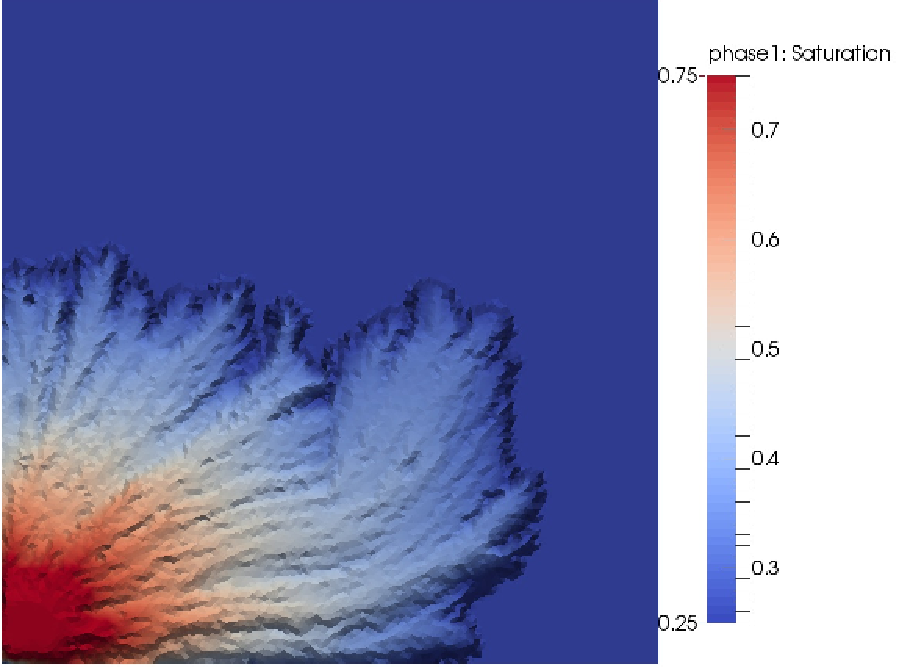
\includegraphics[width=.5\textwidth]{./Pics1/Saffman_heterogeneous_VR10/ST_Heterog_VR10_D11000_W2b.pdf}
       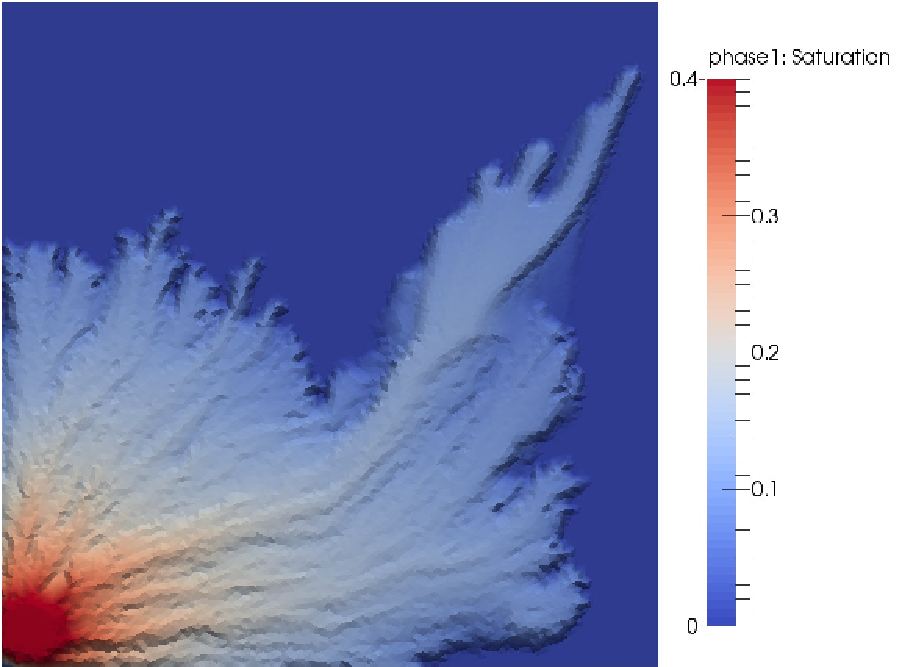
\includegraphics[width=.5\textwidth]{./Pics1/Saffman_heterogeneous_VR150/ST_Heterog_VR150_D6500_W2b.pdf}}
\hbox{\hspace{0.25cm} (c) {\it VR}=10 (heterogeneous) \hspace{1.5cm} (d) {\it VR}=150 (heterogeneous) }
}
\caption{Isosurfaces of simulated flows in Hele-Shaw cells with viscosity ratios of 10 (a and c) and 150 (b and d). Top and bottom rows describe simulations performed with constant \textit{i.e. homogeneous with \textbf{K}}= $10^{-10}$ \textit{${cm}^{2}$} and randomly distributed (i.e. heterogeneous, Fig.~\ref{fig:HeleShawHeter_VR10}a) permeabilities. Width of largest fingers for homogeneous cases are approximately $0.70$ and $0.90$cm (\textit{VR}=$10$ and \textit{VR}=$150$, respectively), whereas for heterogeneous cases are $0.56$ and $0.40$cm. Results for homogeneous cases are in good agreement with values obtained from \citet{guan_2003}'s analytic solution.}
\label{fig:homoheleshaw_VN10_VN150}
\end{figure}
\clearpage



%%%%
%%%%  FIGURE
%%%%
\begin{landscape}
\begin{figure}[ht] 
\vbox{
\hbox{\hspace{4.0cm}
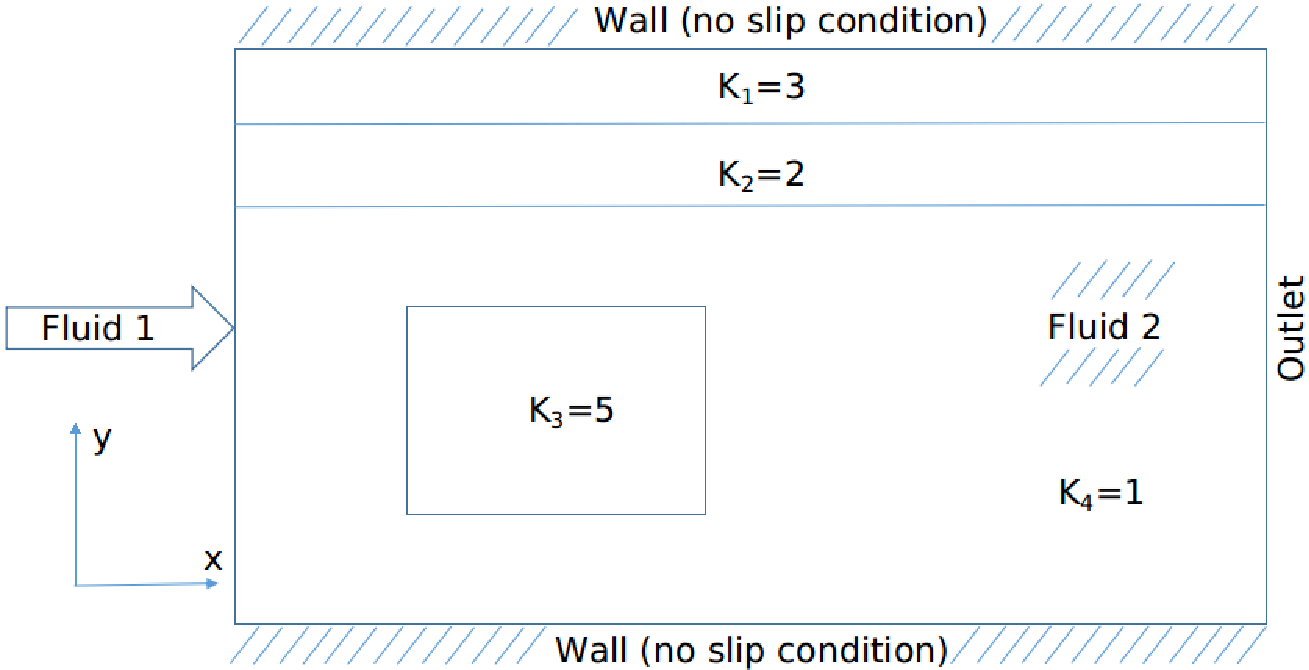
\includegraphics[width=.75\textwidth]{./Pics/map_of_boundaries.pdf} 
}
\vspace{0.0cm}
\hbox{\hspace{6.5cm} (a) map of permeabilties K   
}
\vspace{0.25cm}
\hbox{\hspace{4.0cm}
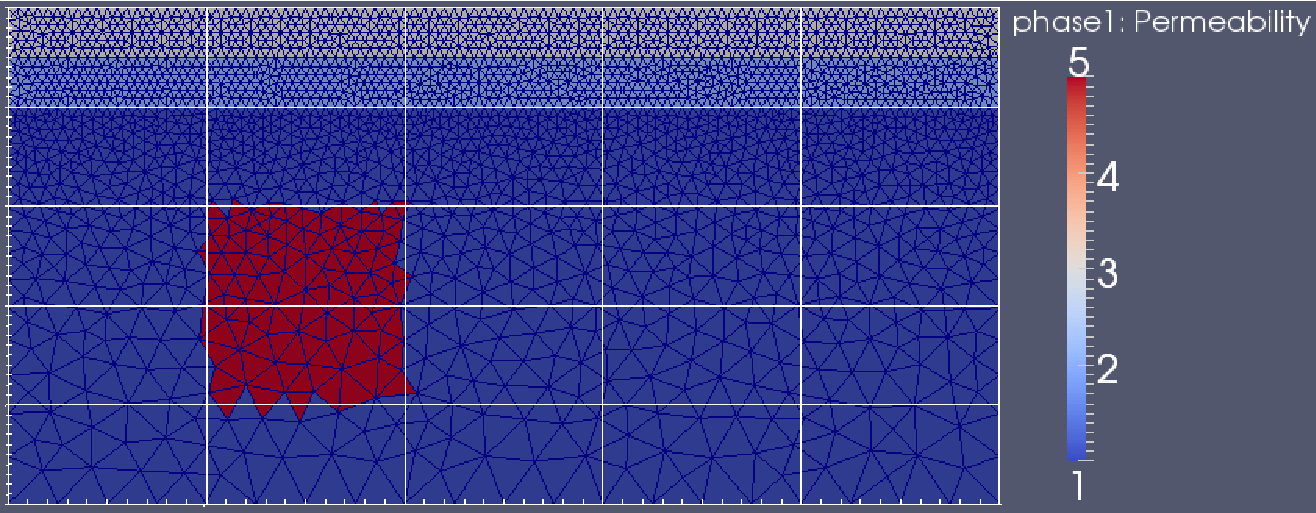
\includegraphics[width=.9\textwidth]{./Pics/map_of_boundaries_1.pdf}
}
\vspace{0.0cm}
\hbox{\hspace{9cm} (b)      
}
}     
\caption{Figure (a) describes the initial and boundary conditions as these are applied in this set of simulations. Below (b) there is a comparison between the unstructured and fixed mesh and the unstructured and adaptive mesh. During the implementation of fixed mesh initially there $4606$ elements while for the adaptive mesh there are $606$ while the majority of them is on the interface between between the two fluids. }
\label{fig:testcase_heter_domain}
\end{figure}
\end{landscape}
\clearpage



%%%
%%% FIGURE
%%%
\begin{landscape}
  \begin{figure}[ht]
    \vbox{ 
      \hbox{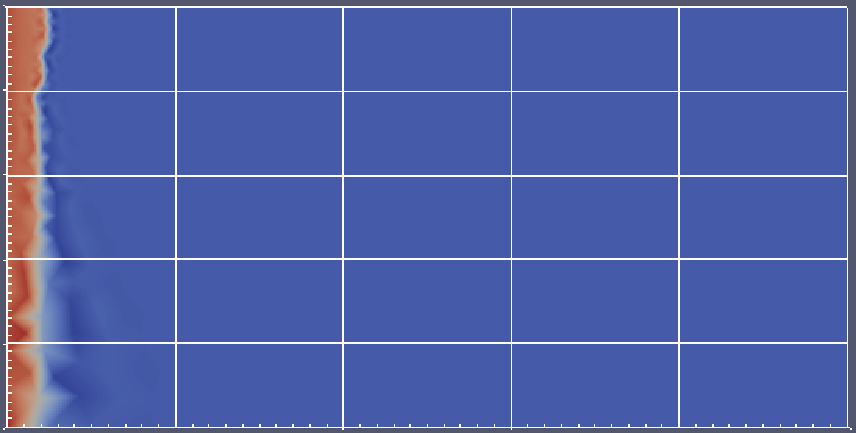
\includegraphics[width=.45\textwidth]{./Pics1/mr1_fixed/mr1_fixed_100_2.pdf}
            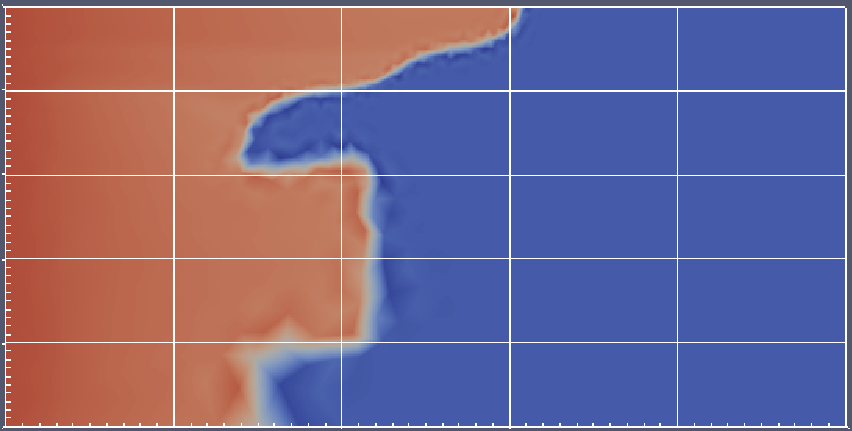
\includegraphics[width=.45\textwidth]{./Pics1/mr1_fixed/mr1_fixed_2500.pdf} 
            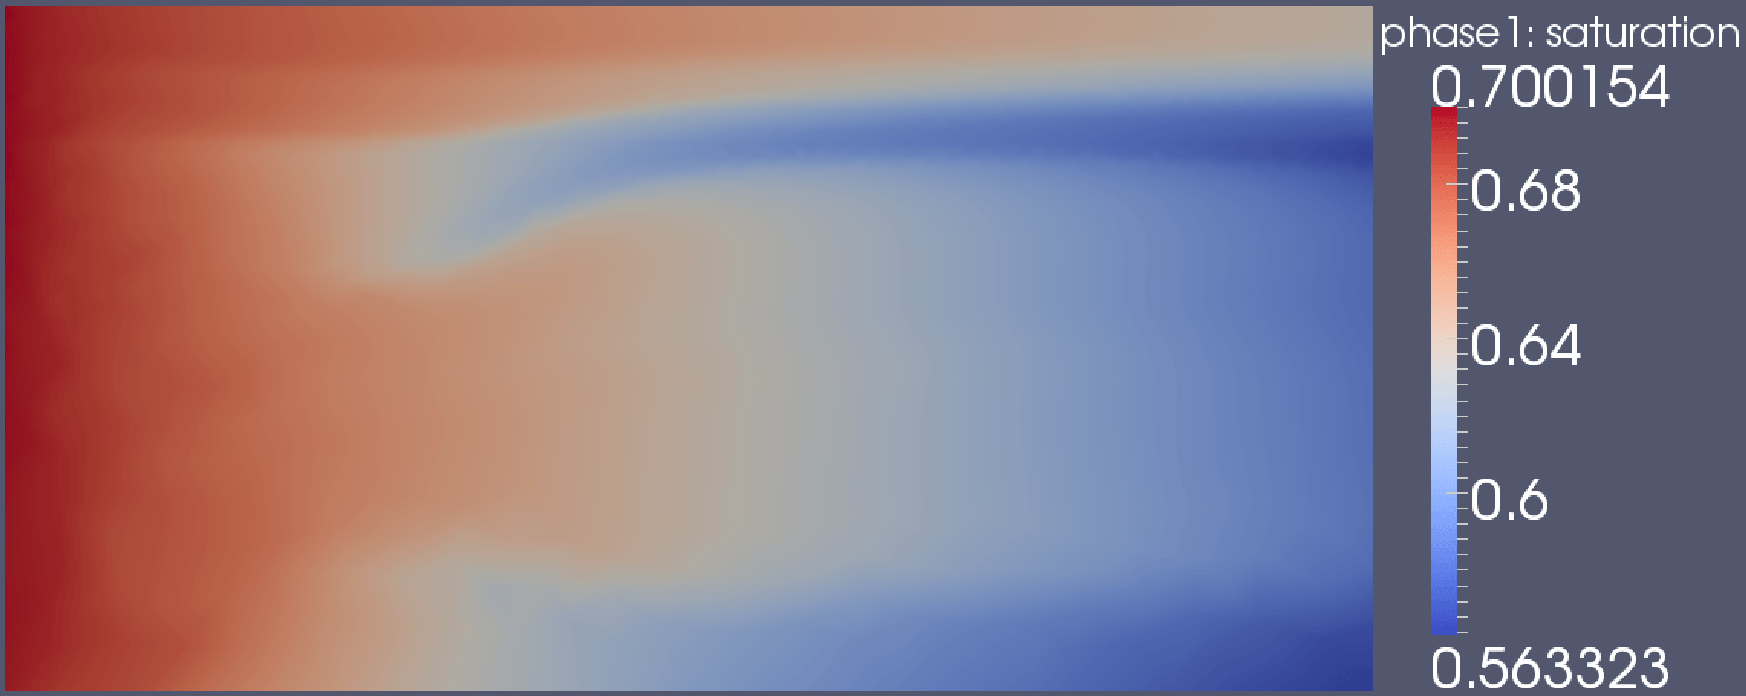
\includegraphics[width=.57\textwidth]{./Pics1/mr1_fixed/mr1_fixed_end_2.pdf} }
      \hbox{\hspace{8.0cm} (a) VR = 1}
      \vspace{1cm}
      \hbox{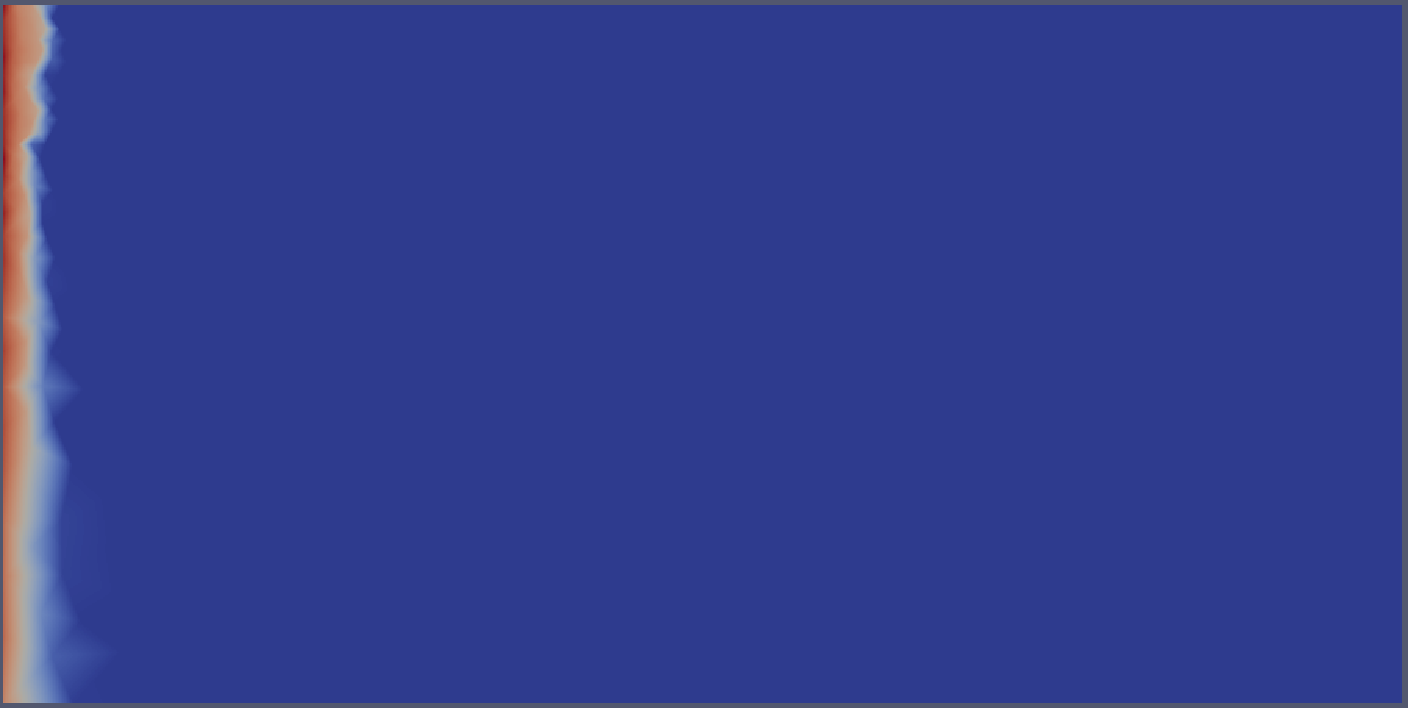
\includegraphics[width=.45\textwidth]{./Pics1/mr10_fixed/mr10_fixed_100_1.pdf}
            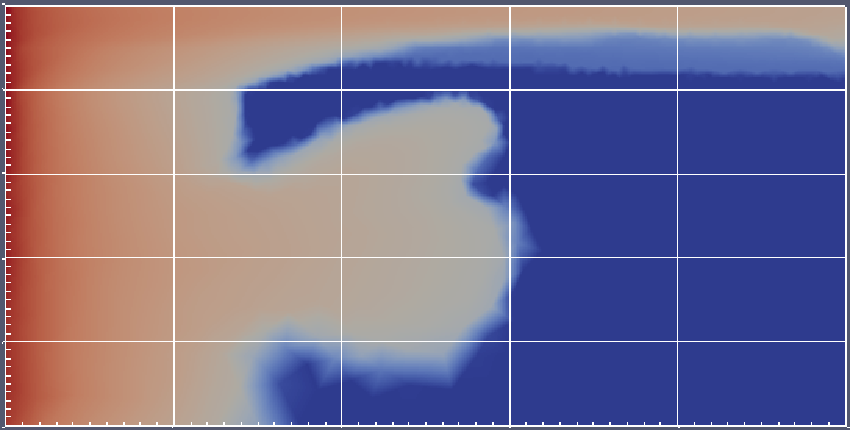
\includegraphics[width=.45\textwidth]{./Pics1/mr10_fixed/mr10_fixed_2500.pdf}
            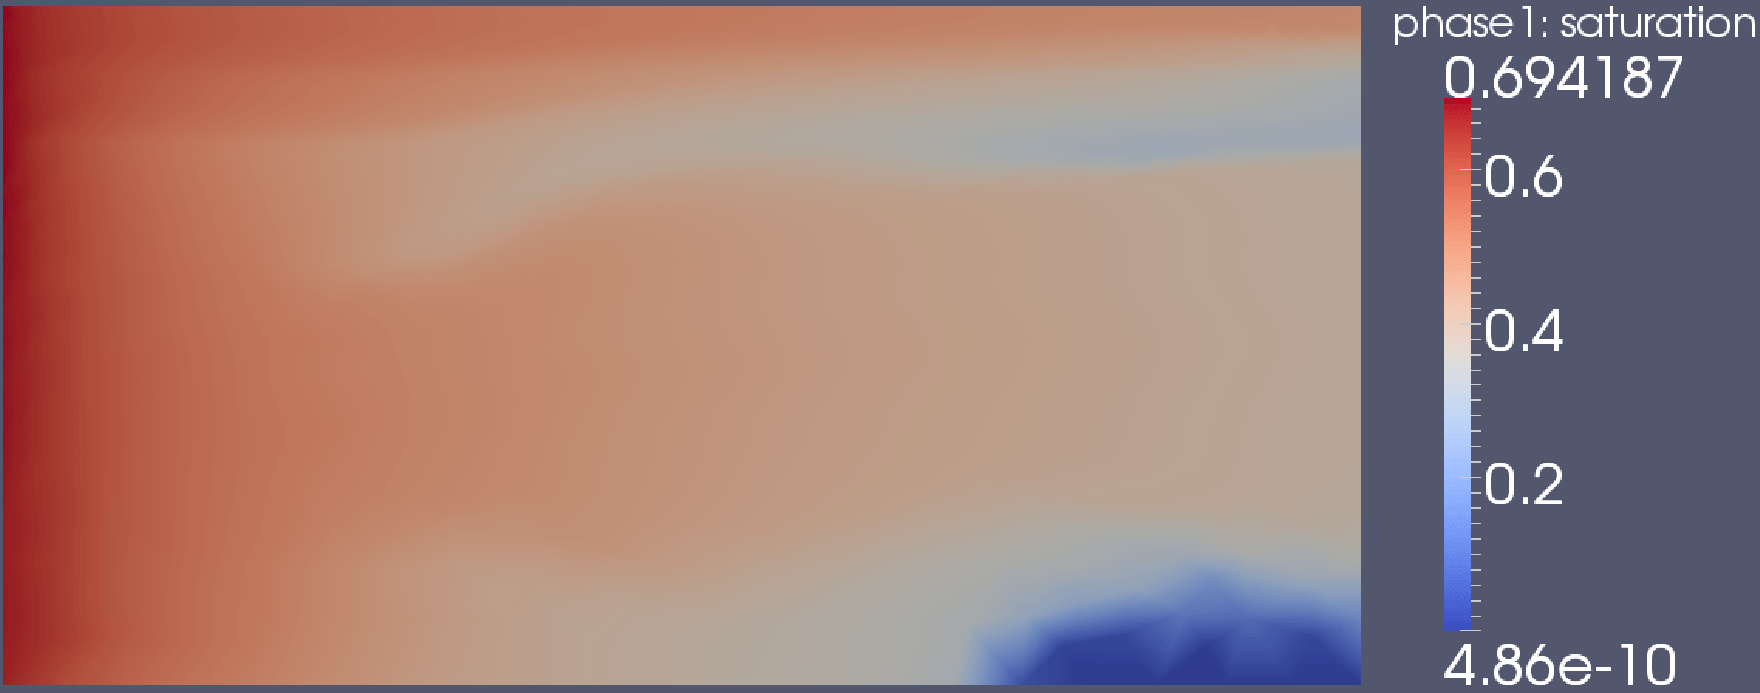
\includegraphics[width=.57\textwidth]{./Pics1/mr10_fixed/mr10_fixed_end_2.pdf} }
      \hbox{\hspace{8.0cm} (b) VR = 10  }}
\caption{Initial model validation: snapshots of numerical simulations performed with VR=1 and VR=10. The domain contains $4678$ elements.(\blue{ Jeff this is a different set of simulation, I have moved it just after the \textit{map of permeabilities} above as a first comparison between $VR1$ and $VR10$})}
\label{fem_cv_represent_vr1_vr10}
\end{figure}
\end{landscape}
\clearpage
%%%
%%%
%%%



%%%%
%%%%  FIGURE
%%%%
\begin{landscape}
\begin{figure}[ht] 
\vbox{
\hbox{\hspace{3.5cm}
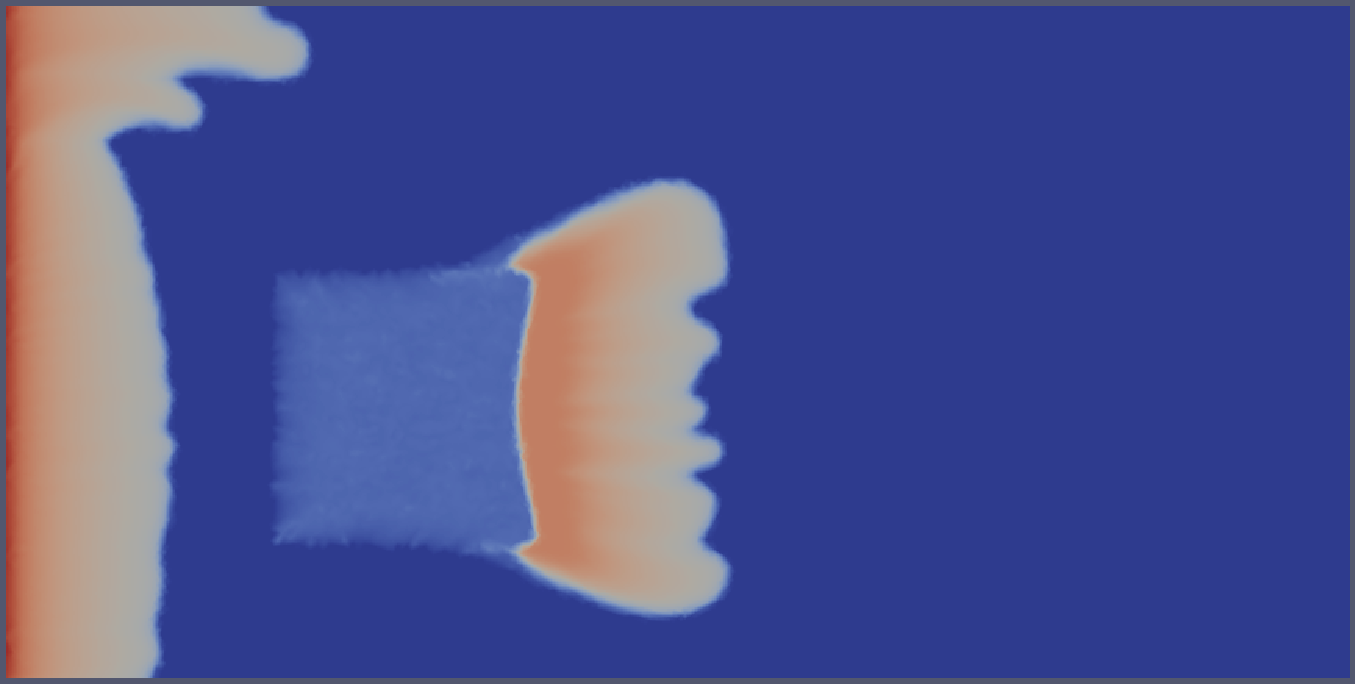
\includegraphics[width=.65\textwidth]{./Pics1/mr10_5regions_fixed/5regions_fixed_250.pdf} 
}
\vspace{0.0cm}
\hbox{\hspace{6.5cm} (a) flow at t=250 (fixed mesh)  
}
\vspace{0.25cm}
\hbox{\hspace{3.5cm}
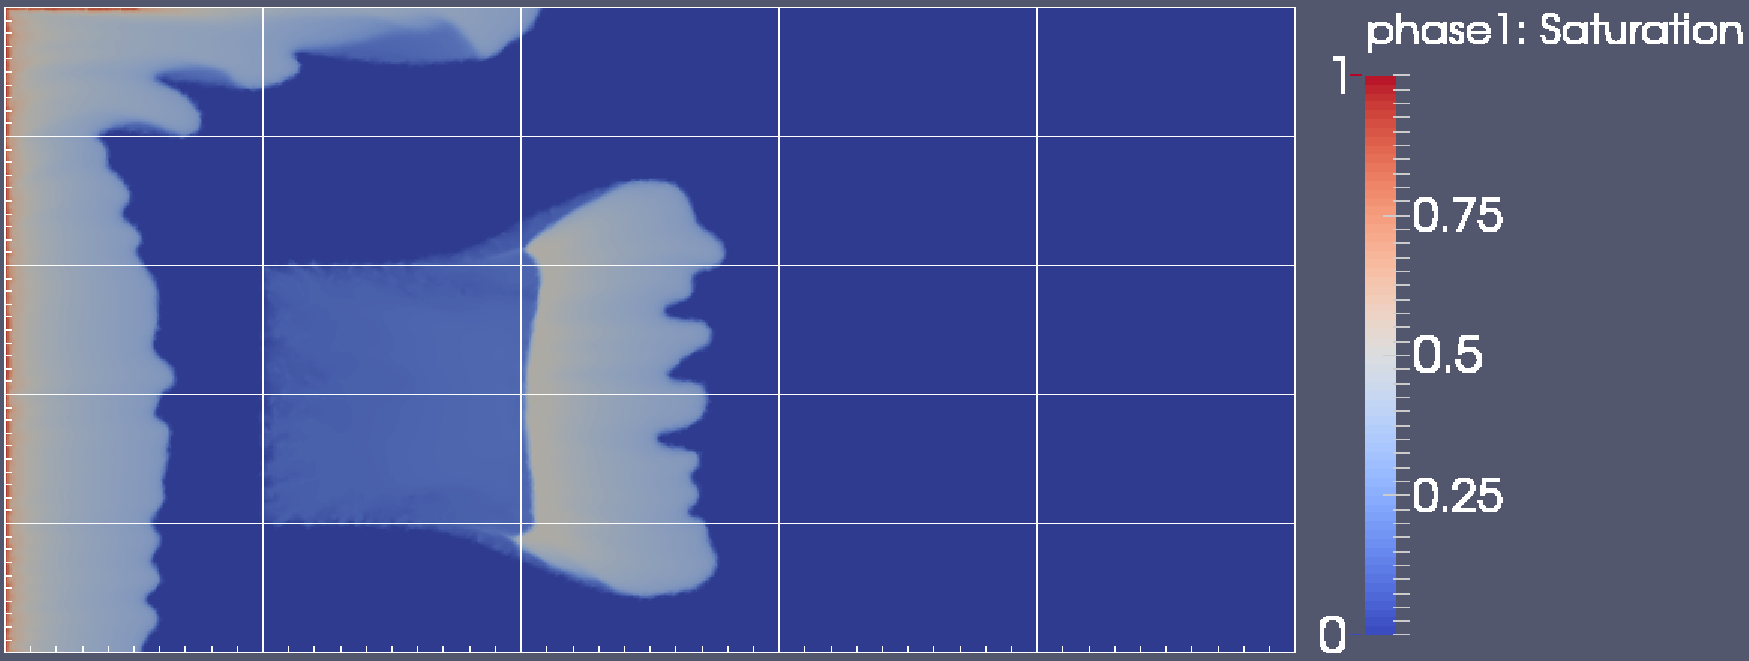
\includegraphics[width=.9\textwidth]{./Pics1/mr10_5regions_adapt/5regions_adapt_250_1.pdf}
}
\vspace{0.0cm}
\hbox{\hspace{6.5cm} (b) flow at t=250 (adaptive mesh)    
}
}     
\caption{For $t=0.125$s, $2$ test-cases under the VR=$10$ and under fixed (top) and adaptive(bottom) mesh are compared. There is a significant difference on the main front (left hand side of the domain) and the number of finger that appear.}
\label{fig:2testcase_a}
\end{figure}
\end{landscape}
\clearpage



%%%%
%%%%  FIGURE
%%%%
\begin{landscape}
\begin{figure}[ht] 
\vbox{
\hbox{\hspace{3.5cm}
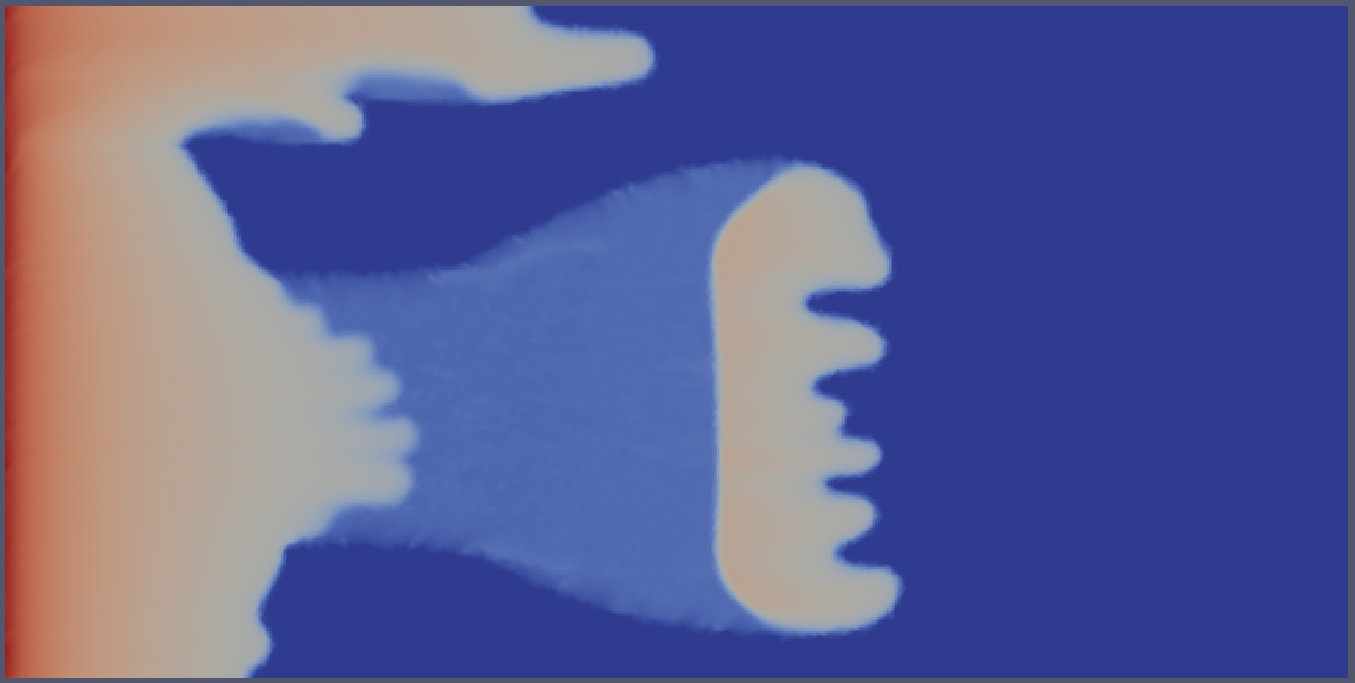
\includegraphics[width=.65\textwidth]{./Pics1/mr10_5regions_fixed/5regions_fixed_500.pdf} 
}
\vspace{0.0cm}
\hbox{\hspace{6.5cm} (a) flow at t=500 (fixed mesh)   
}
\vspace{0.25cm}
\hbox{\hspace{3.5cm}
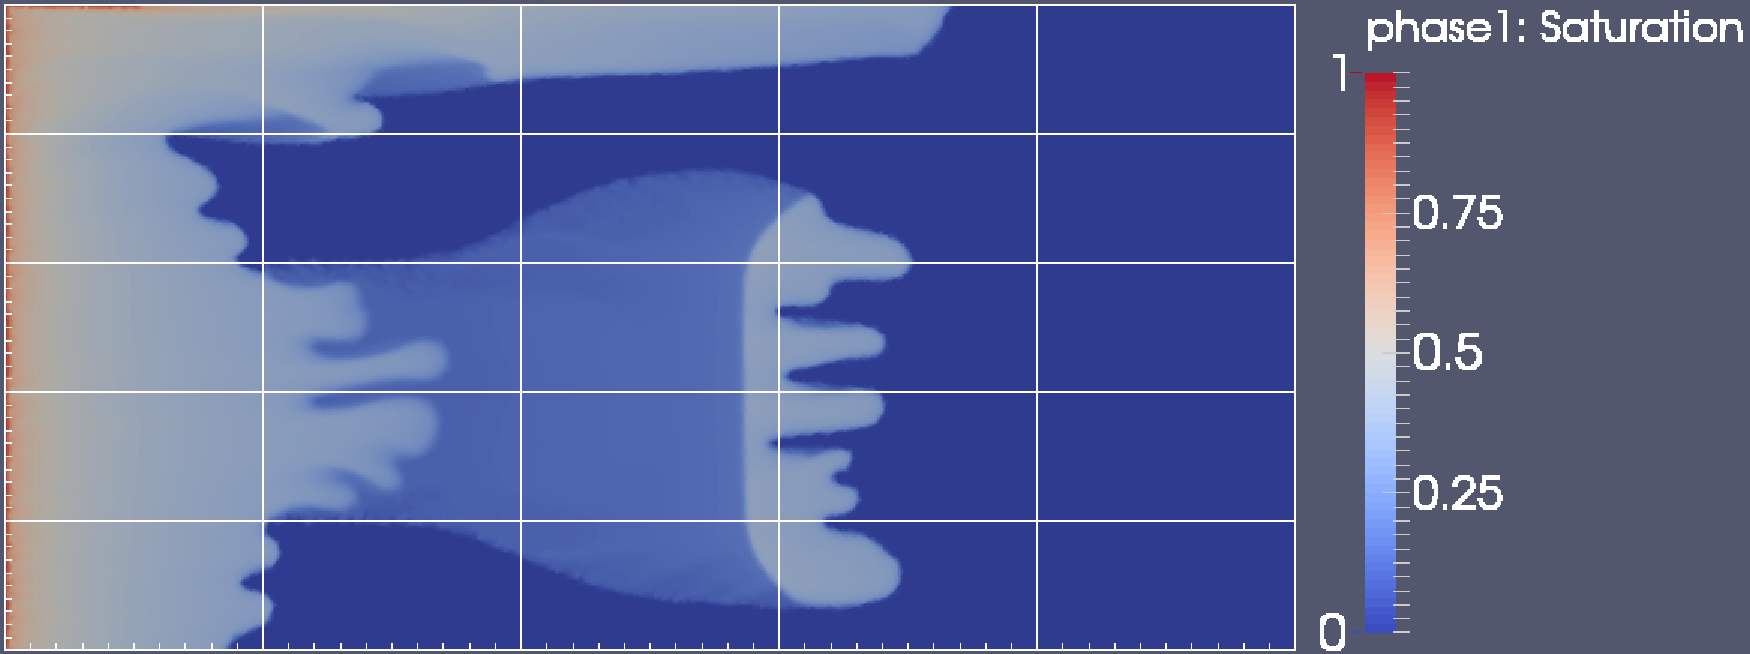
\includegraphics[width=.9\textwidth]{./Pics1/mr10_5regions_adapt/5regions_adapt_500_1.pdf}
}
\vspace{0.0cm}
\hbox{\hspace{6.5cm} (b) flow at t=500 (adaptive mesh)     
}
}     
\caption{At $t=0.25$s ($t=500$, timestemp) cross flow is taking place at the upper part of the formation. The fingers start to becoming more proufound as can been seen at the bottom.}
\label{fig:2testcase_b}
\end{figure}
\end{landscape}
\clearpage



%%%%
%%%%  FIGURE
%%%%
\begin{landscape}
\begin{figure}[ht] 
\vbox{
\hbox{\hspace{3.5cm}
\includegraphics[width=.65\textwidth]{./Pics1/mr10_5regions_fixed/5regions_fixed_1500.pdf} 
}
\vspace{0.0cm}
\hbox{\hspace{6.5cm} (a) flow at t=1500 (fixed mesh)   
}
\vspace{0.25cm}
\hbox{\hspace{3.5cm}
\includegraphics[width=.9\textwidth]{./Pics1/mr10_5regions_adapt/5regions_adapt_1500_1.pdf}
}
\vspace{0.0cm}
\hbox{\hspace{6.5cm} (b) flow at t=1500 (adaptive mesh)     
}
}     
\caption{At $t=0.75 sec$ ($t=1500$, timestemp) the initial cross flow is now fully developed and has travel all the way towards the outlet (right-hand side). and the finger below start forming a front that is also travelling towards the left-hand side.}
\label{fig:2testcase_c}
\end{figure}
\end{landscape}
\clearpage



%%%%
%%%%  FIGURE
%%%%
\begin{landscape}
\begin{figure}[ht] 
\vbox{
\hbox{\hspace{3.5cm}
\includegraphics[width=.65\textwidth]{./Pics1/mr10_5regions_fixed/5regions_fixed_2000.pdf} 
}
\vspace{0.0cm}
\hbox{\hspace{6.5cm} (a) flow at t=end (fixed mesh)   
}
\vspace{0.25cm}
\hbox{\hspace{3.5cm}
\includegraphics[width=.9\textwidth]{./Pics1/mr10_5regions_adapt/5regions_adapt_3000_1.pdf}
}
\vspace{0.0cm}
\hbox{\hspace{6.5cm} (b) flow at t=end (adaptive mesh)     
}
}     
\caption{Using the $P_{1}DGP_{2}$ element type for VR=$10$ under the same time steps, we compared the impact of fixed and adaptive mesh for the same timeframe. The end of simulation happens at $time=5 sec$ and for the timestemp $t=9999$ while the number of elements in both simulations was approximately $4700$. When adaptive mesh is introduce there is better repersentation of the fluid instabilities as these are developed on time.}
\label{fig:2testcase_d}
\end{figure}
\end{landscape}
\clearpage



%%%%
%%%%  FIGURE
%%%%
\begin{landscape}
\begin{figure}[ht] 
\vbox{
\hbox{\hspace{3.5cm}
\includegraphics[width=.9\textwidth]{./Pics1/mr10_5regions_fixed_dinlet/5regions_dinlet_fixed_100_1.pdf}
}
\vspace{0.0cm}
\hbox{\hspace{6.5cm} (a) double inlet - fixed mesh   
}
\hbox{\hspace{3.5cm}
  \includegraphics[width=.67\textwidth]{./Pics1/mr10_5regions_adapt_dinlet/5regions_dinlet_adapt_start.pdf}
}
\vspace{0.0cm}
\hbox{\hspace{6.5cm} (b) double inlet adaptive mesh   
}
}     
\caption{Comparing test-cases of fixed and adaptive mesh while a second region/inlet is introduced. For $t=0.101$s, using the $P_{1}DGP_{2}$ element type for MR=$10$ under the same time steps. For this simulation there are $13226$ elements for the fixed messh and $43716$ for the adaptive.}
\label{fig:3testcase_a}
\end{figure}
\end{landscape}
\clearpage

%%%%
%%%%  FIGURE
%%%%
\begin{landscape}
\begin{figure}[ht] 
\vbox{
\hbox{\hspace{3.5cm}
\includegraphics[width=.65\textwidth]{./Pics1/5reg_dinlet_fixed_500.pdf} 
}
\vspace{0.0cm}
\hbox{\hspace{6.5cm} (a) double inlet - fixed mesh   
}
\hbox{\hspace{3.5cm}
\includegraphics[width=.9\textwidth]{./Pics1/5reg_dinlet_adapt_500_1.pdf}
}
\vspace{0.0cm}
\hbox{\hspace{6.5cm} (b) double inlet adaptive mesh   
}
}     
\caption{For $t=5$s there is a comparison between fixed mesh(a) and adaptive mesh(b).}
\label{fig:3testcase_b}
\end{figure}
\end{landscape}
\clearpage

%%%%
%%%%  FIGURE
%%%%
\begin{landscape}
\begin{figure}[ht] 
\vbox{
\hbox{\hspace{3.5cm}
\includegraphics[width=.65\textwidth]{./Pics1/5reg_dinlet_fixed_1500.pdf} 
}
\vspace{0.0cm}
\hbox{\hspace{6.5cm} (a) double inlet - fixed mesh   
}
\hbox{\hspace{3.5cm}
\includegraphics[width=.9\textwidth]{./Pics1/5reg_dinlet_adapt_1500_1.pdf}
}
\vspace{0.0cm}
\hbox{\hspace{6.5cm} (b) double inlet adaptive mesh   
}
}     
\caption{For $t=7.5$s this is a comparison between fixed mesh(a) and adaptive mesh(b).}
\label{fig:3testcase_c}
\end{figure}
\end{landscape}
\clearpage

%%%%
%%%%  FIGURE
%%%%
\begin{landscape}
\begin{figure}[ht] 
\vbox{
\hbox{\hspace{3.5cm}
\includegraphics[width=.65\textwidth]{./Pics1/5reg_dinlet_fixed_end.pdf} 
}
\vspace{0.0cm}
\hbox{\hspace{6.5cm} (a) double inlet - fixed mesh   
}
\hbox{\hspace{3.5cm}
\includegraphics[width=.9\textwidth]{./Pics1/5reg_dinlet_adapt_end_1.pdf}
}
\vspace{0.0cm}
\hbox{\hspace{6.5cm} (b) double inlet adaptive mesh   
}
}     
\caption{This is a comparison between fixed mesh(a) and adaptive mesh(b) at the end of the simulation. For the fixed mesh at this point the maximum number of point is $13226$ while for the adaptive mesh is $7582$ and most of them are located where is needed in the domain.}
\label{fig:3testcase_d}
\end{figure}
\end{landscape}
\clearpage

%%%%
%%%%  FIGURE
%%%%
\begin{landscape}
\begin{figure}[ht] 
\vbox{
\hbox{\hspace{3.5cm}
\includegraphics[width=.93\textwidth]{./Pics1/mr100_fixed/mr100_fixed_500.pdf} 
}
\vspace{0.0cm}
\hbox{\hspace{4.0cm} (a) fixed and unstructured mesh for VR = 100 (start)   
}
\hbox{\hspace{3.5cm}
\includegraphics[width=.7\textwidth]{./Pics1/mr100_fixed/mr100_fixed_1500.pdf}
}
\vspace{0.0cm}
\hbox{\hspace{3.75cm} (b) fixed and unstructured mesh for VR = 100 (t = 1500)   
}
}     
\caption{For the case of VR=$100$ from top to bottom, the number of elements is $4680$ and fixed and unstructured mesh was used for the same time steps, t=$0.25$s or t=500(a), t=$0.75$s or t=1500(b). }
\label{fig:4testcase_a}
\end{figure}
\end{landscape}
\clearpage

%%%%
%%%%  FIGURE
%%%%
\begin{landscape}
\begin{figure}[ht] 
\vbox{
\hbox{\hspace{3.5cm}
\includegraphics[width=.7\textwidth]{./Pics1/mr100_fixed/mr100_fixed_3000.pdf} 
}
\vspace{0.0cm}
\hbox{\hspace{3.75cm} (c) fixed and unstructured mesh for VR = 100    
}
\hbox{\hspace{3.5cm}
\includegraphics[width=.93\textwidth]{./Pics1/mr100_fixed/mr100_fixed_end.pdf}
}
\vspace{0.0cm}
\hbox{\hspace{7.cm} (d) end of simulations     
}
}     
\caption{screenshot (c) is for t=$1.5$s or t=$3000$ and screenshot (d) is for t=$3.175$s, at the end of the simulations. }
\label{fig:4testcase_b}
\end{figure}
\end{landscape}
\clearpage



%%%
%%% FIGURE XXXXXX
%%%
\begin{figure}[ht]
\vbox{\vspace{-.5cm}
      \hbox{\includegraphics[width=\textwidth]{./Pics1/3D_Channel/Test_SlowNew_MeshPermeability.pdf} }
      \hbox{\hspace{5.0cm} (a) permeability map }}
\caption{3D channel flow. The domain contains 243056 \PN[1]{1} element-pairs.}
\label{fig:3DChannel_PermMesh}
\end{figure}
\clearpage

%%%%
%%%%  FIGURE
%%%%
\begin{landscape}
\begin{figure}[ht] 
\vbox{
\hbox{\hspace{3.5cm}
\includegraphics[width=1.0\textwidth]{./Pics1/3D_Channel/3D_channel_darcy_vel_planes_100.pdf} 
}
\vspace{0.0cm}
\hbox{\hspace{10.0cm} (a)     
}
\hbox{\hspace{3.5cm}
\includegraphics[width=1.0\textwidth]{./Pics1/3D_Channel/3D_channel_darcy_vel_planes_490.pdf}
}
\vspace{0.0cm}
\hbox{\hspace{10.cm} (b)      
}
}     
\caption{ contours of Darcy velocity in XY and YZ planes for (a) t=$0.91$s and (b)t=$4.3$s.}
\label{fig:3DChannel_darcy_vel}
\end{figure}
\end{landscape}
\clearpage

%%%%
%%%%  FIGURE
%%%%
\begin{landscape}
\begin{figure}[ht] 
\vbox{
\hbox{\hspace{3.5cm}
\includegraphics[width=1.0\textwidth]{./Pics1/3D_Channel/3D_channel_sat_100.pdf} 
}
\vspace{0.0cm}
\hbox{\hspace{10.0cm} (a)     
}
\hbox{\hspace{3.5cm}
\includegraphics[width=1.0\textwidth]{./Pics1/3D_Channel/3D_channel_sat_490.pdf}
}
\vspace{0.0cm}
\hbox{\hspace{10.cm} (b)      
}
}     
\caption{For the same time steps as in fig.\ref{fig:3DChannel_darcy_vel} there is a description of the saturation front in (a) t=$0.91$s and (b)t=$4.3$s.}
\label{fig:3DChannel_sat}
\end{figure}
\end{landscape}
\clearpage




